\documentclass[11pt,a4paper]{article}

\usepackage[margin=1.1in]{geometry}
\usepackage{amsmath,amssymb,amsthm,mathtools}
\usepackage[T1]{fontenc}
\usepackage{palatino}
\usepackage{microtype}
\microtypesetup{expansion=false,protrusion=true}
\usepackage{tikz}
\usetikzlibrary{positioning,arrows.meta,calc,fit,backgrounds,patterns}
\usepackage{booktabs}
\usepackage{listings}
\usepackage{stmaryrd}
\usepackage[hidelinks]{hyperref}
\usepackage{enumitem}

\setlength{\emergencystretch}{2.5em}

\theoremstyle{plain}
\newtheorem{theorem}{Theorem}
\newtheorem{proposition}[theorem]{Proposition}
\newtheorem{lemma}[theorem]{Lemma}
\newtheorem{corollary}[theorem]{Corollary}
\newtheorem{conjecture}[theorem]{Conjecture}
\theoremstyle{definition}
\newtheorem{definition}[theorem]{Definition}
\newtheorem{observation}[theorem]{Observation}
\newtheorem{principle}[theorem]{Principle}
\newtheorem{question}[theorem]{Question}
\theoremstyle{remark}
\newtheorem{remark}[theorem]{Remark}

\newcommand{\Open}{\mathsf{Open}}
\newcommand{\Ebox}{\exists\Box}
\newcommand{\gE}[2]{\langle E\rangle^{#1}_{#2}}
\newcommand{\gK}[1]{\langle K_{#1}\rangle}
\newcommand{\Nsp}{\mathcal{N}}
\newcommand{\Val}{V}
\newcommand{\sem}[1]{\llbracket #1 \rrbracket}
\newcommand{\tv}{\mathbf{t}}
\newcommand{\fv}{\mathbf{f}}
\newcommand{\bv}{\mathbf{b}}
\newcommand{\nil}{\mathbf{0}}
\newcommand{\inn}[3]{\mathrm{for}(#1 \leftarrow #2)\,#3}
\newcommand{\qq}[1]{@#1}
\newcommand{\sep}[2]{\mathbin{\big|^{#1}_{#2}}}
\newcommand{\Cand}{\mathrm{Cand}}
\newcommand{\Fml}{\mathrm{Fml}}

\lstset{basicstyle=\ttfamily\small,columns=fullflexible,breaklines=true,
        keepspaces=true,showstringspaces=false,xleftmargin=1.2em}

\title{\bfseries Quorum as a Where-Clause\\[4pt]
\large Coalition Logic as a graded hypothesis language for populations of
computations,\\
with a swarm that decides and a pride that reads}

\author{L. Gregory Meredith\\
\small F1R3FLY.io / F1R3FLY Industries\\
\small \texttt{lgreg.meredith@gmail.com}}

\date{Research Note --- August 2026}

\begin{document}
\maketitle

\begin{abstract}
A companion note read Gabbay's Coalition Logic as a declarative specification
language whose proofs, under a Curry--Howard term assignment, extract rho
calculus implementations of consensus protocols. This note reads the same logic
in the other direction, as the hypothesis language of a computation trying to
predict a population of computations in its environment. The coalition modality
$\Ebox$ is placed in the \emph{where}-clause of a rho for-comprehension and
graded over a resolution semiring, joining the context-labelled behavioural
modality $\gK{j}$ already used by the mortal scientist. The observational route
needs only the model theory of Coalition Logic, which exists, and not its proof
theory, which does not.

We work two examples. The first is a honeybee swarm choosing a nest site, where
the observer is \emph{inside} the population: a scout sensing a quorum at a
cavity is evaluating the coalition modality about her own swarm, and her verdict
is what triggers the swarm's commitment. This case has four decades of
measurement behind it, and the framework makes contact with it in three ways
--- it derives Seeley's quorum-versus-consensus finding from an altitude
argument rather than assuming it, it predicts a structural threshold at twice
the quorum size across which the job of cross-inhibitory stop signalling
changes from breaking deadlock to preventing splits, and it predicts that
quorum-sensing errors are one-sided with the apparent threshold scaling in
cavity geometry. The second example is a lion pride reading a stampeding herd,
where the observer is \emph{outside}; it is simulated rather than measured, and
it isolates results the internal case cannot show: that the coalition modality
buys irreversibility rather than accuracy, and that a population resists being
read by denying its observer coverage rather than by inducing error --- losing
its own capacity to agree in the same move.

Across both: quorum intersection, the safety property of consensus, is what
makes a population legible at all; and a mortal observer cannot distinguish a
faulty participant from an observation it could not afford to finish.
\end{abstract}

\tableofcontents

\section{Introduction}\label{sec:intro}

A swarm of honeybees hangs on a branch. Several hundred of its ten thousand
workers are scouting the surrounding countryside for a cavity to live in, and
over the next day or two the swarm will commit to one of them --- irrevocably,
and with no bee anywhere in possession of a global tally. What settles it, as
Seeley and Visscher established, is not agreement among the dancers back at the
cluster but a \emph{quorum} sensed at a cavity: when enough scouts are present
at one site, the scouts there return and pipe, the cluster warms up, and the
swarm flies \cite{SV04,Seeley10}.

A lion pride is stalking a herd. The herd startles, and in the next few seconds
it will break --- left or right, as one body or in fragments. The pride's entire
investment turns on committing to the correct flank before the break completes.
It is not trying to \emph{make} the herd break left; it is trying to
\emph{know} that the herd has already decided to.

These are the same question asked from two positions. In both, a computation
wants to know whether a population of computations has reached a conclusion. In
the swarm the asker is a member of the population and her verdict causes the
conclusion to take effect; in the pride the asker is outside and can only watch.
The first case has hard data behind it and is the centre of this note; the
second is simulated, and earns its place by isolating things the first cannot
show.

The companion note \cite{consensus} observed that Gabbay's Coalition Logic
\cite{GZ25,Gab25}, interpreted over semitopologies \cite{Gab23,Gab24}, is a
declarative language for distributed agreement, and proposed a Curry--Howard
correspondence under which proofs of Coalition Logic formulae are decorated with
rho calculus terms carrying join patterns, so that
\[
\mathrm{for}(y_1 \leftarrow x_{p_1}\ \&\ \cdots\ \&\ y_n \leftarrow x_{p_n})\,P
\]
witnesses the coalition modality $\Ebox\varphi$. That is a synthesis programme:
from specification to correct-by-construction implementation.

The present note runs the same correspondence backwards. Neither the scout nor
the pride wants a term realising $\Ebox\varphi$; each wants to evaluate whether
$\Ebox\varphi$ \emph{holds} of a population it did not write. We are on the
satisfaction side of the turnstile rather than the derivation side, and the
computational vehicle is not a proof but a guard.

Three commitments organise the note.

\paragraph{The clause is the vehicle.} Recent work \cite{gradedwhere,choicef}
developed the \emph{graded where-clause}: the rho for-comprehension
$\mathrm{for}(y \leftarrow x \ \mathbf{where}\ \psi)$ whose guard is not a
Boolean but a value in a resolution semiring, keyed by spatial-behavioural
formulae. A clause weighs the candidates in a fibre; it does not select from
it. We add the coalition modality to the clause language. In the swarm the
distinction between weighing and selecting is not a technicality but two
different behaviours performed by two different sets of bees.

\paragraph{The semitopology is the hypothesis.} In Gabbay's setting a model
\emph{is} a semitopology $(P,\Open)$: the collection of actionable coalitions
is given with the model. Neither a scout nor a pride has such access. Their
$\Open$ is a conjecture, and the relaxation lattice of \cite{scientist} orders
conjectures, so the machinery for revising a guessed semitopology is already
built.

\paragraph{Everything is priced.} The problem is not merely to be right but to
be right \emph{cheaply} and \emph{early}. We therefore work in cost-accounted
rho \cite{costmonad}, price each hypothesis, and report yields.

\subsection{What is new here}

Against \cite{consensus}: the direction of the correspondence, the grading, the
behavioural modality $\gK{j}$, the discovery of $\Open$, and cost. Against
\cite{scientist,game,compose}: the object of study is a \emph{population}
rather than an individual, and the logic acquires a modality quantifying over
coalitions rather than over redex positions. Against \cite{gradedwhere,choicef}:
a second modality in the same clause, and a use of the graded machinery which is
observational rather than resolutive --- except in the swarm, where the two
coincide, and which is therefore the first worked instance of the resolutive
reading those notes left open.

Against the honeybee literature the position is more delicate and is stated at
the head of \S\ref{sec:swarm}. There is a mature quantitative modelling
tradition here --- leaky competing accumulators, value-sensitive decision
dynamics, best-of-$n$ analyses \cite{Seeley12,Pais13,Reina17} --- and nothing
below out-predicts it on trajectories. What the framework contributes is a logic
for \emph{what} a scout is testing, a cost argument for why she tests that and
not something else, and structural impossibility results that a statistical
model is not in a position to state.

\subsection{Results}

\begin{itemize}[leftmargin=1.4em]
\item The satisfaction reading needs only the model theory of Coalition Logic.
      Problems P1--P5 of \cite{consensus} --- the missing sequent calculus, cut
      elimination, subject reduction for the term assignment, adequacy --- are
      all on the synthesis side and are not obstacles here
      (\S\ref{sec:reversal}).
\item Section 7.1 of \cite{consensus} contrasts decomposition over
      \emph{participants} with decomposition over \emph{process structure}. In
      a reflective calculus this contrast collapses: participants are
      processes, names are quotations of processes, and open-set quantification
      is separating conjunction at a different index
      (Proposition~\ref{prop:collapse}).
\item Over $\mathbb{R}_{\ge 0}$ with multiplicative $\otimes$, larger coalitions
      score \emph{weaker}, which is the wrong semantics for a quorum. The
      correct algebras are tropical and Viterbi, where the coalition value is
      the strength of the weakest member --- and these are exactly the two
      algebras in which the attainment proposition of \cite{choicef} holds on
      the nose, so the observer receives a \emph{witness coalition} and not
      merely a number (\S\ref{sec:algebra}).
\item A mortal observer cannot distinguish Gabbay's third truth value $\bv$, a
      property of the participant, from its own exhausted budget, a property of
      the observation (Proposition~\ref{prop:twobottoms}).
\item Quorum intersection --- $2$-twinedness, Gabbay's \emph{safety} condition
      --- is what makes a population legible. Under it the population has at
      most one conclusion, so the observer's hypothesis is a function
      (Proposition~\ref{prop:functional}).
\end{itemize}

\noindent From the swarm (\S\ref{sec:swarm}):
\begin{itemize}[leftmargin=1.4em]
\item Quorum-sensing at a site and consensus-sensing at the cluster are
      different formulae at different altitudes: the first is a local
      $\bigoplus\bigotimes$ over one open, the second a global universal. No
      bee can evaluate a global universal within its access grades, so the
      framework \emph{derives} the finding of \cite{SV04}
      (Proposition~\ref{prop:whyquorum}).
\item \textbf{The $2k$ theorem.} Two simultaneous quorums require $2k$
      committed scouts, so a swarm whose active scout pool falls short of twice
      the quorum threshold cannot split, whatever the site qualities and
      whatever the stop signalling (Theorem~\ref{thm:twok}). Measured: splits
      are identically $0.0000$ at every $S < 30$ and first appear at $S = 30$
      with $k = 15$.
\item \textbf{Cross-inhibition changes jobs at $S = 2k$.} Below the threshold
      the failure mode is deadlock and stop signalling removes it entirely
      ($0.5120 \to 0.0000$ at $S = 16$); above it the failure mode is splitting
      and stop signalling only mitigates it ($0.3860 \to 0.1170$ at $S = 40$).
      This is a discriminating prediction: the two accounts of what stop
      signals are for should be separable by manipulating the scout pool
      (\S\ref{sec:twok}).
\item \textbf{Quorum errors are one-sided, and the threshold is not a number.}
      If a scout senses quorum by encounter rate, false positives are
      structurally impossible and the \emph{apparent} threshold in bees scales
      linearly with cavity geometry: measured $16, 21, 25, 33$ true bees for
      effective areas $1, 1.25, 1.5, 2$ against a nominal $k = 15$
      (\S\ref{sec:onesided}).
\end{itemize}

\noindent From the pride (\S\ref{sec:worked}--\S\ref{sec:topen}):
\begin{itemize}[leftmargin=1.4em]
\item The coalition modality does not buy accuracy; it buys
      \emph{irreversibility}. Over $6839$ coalition verdicts the precision was
      $1.0000$ at every observation time, while a five-animal sample ranged
      from $0.9160$ to $0.9873$. The cost of the coalition rung is $19\times$
      the sample's and its folded accuracy is \emph{lower}
      (\S\ref{sec:ladder}).
\item A population defends itself against being read not by deceiving the
      observer but by denying it coverage. As the herd's internal seams grow
      from $0$ to $6$, the pride's coverage falls from $0.7520$ to $0.0115$
      while its precision stays at $1.0000$ --- safety preserved, liveness
      lost. The herd pays in its own consensus, which falls from $0.7257$ to
      $0.2331$ (\S\ref{sec:countermove}).
\item Grading at the coalition size is crisp in disguise: $\min$ over thirteen
      animals is zeroed by one dissenter, and the crisp and graded rungs return
      identical verdicts. The grading pays only when the coalition size is
      \emph{relaxed} at the same time --- at which point the margin becomes a
      clock. Both examples show this, with waits falling monotonically across
      margin quartiles: $42.4, 29.6, 28.9, 18.0$ ticks for the herd and
      $59.7, 35.1, 18.4, 8.4$ for the swarm (\S\ref{sec:clock}).
\end{itemize}

Every number is computed by \texttt{swarm.py} and \texttt{herd.py}, described
in Appendix~\ref{app:computations}.

\section{What is imported}\label{sec:imported}

We assume, and do not restate, the following.

\paragraph{From \cite{consensus}.} Semitopologies $(P,\Open)$, where $\Open$
contains $\emptyset$ and $P$ and is closed under arbitrary unions but
\emph{not} under finite intersection; points are participants and opens are
actionable coalitions. Semiframes and the compatibility relation $*$. Coalition
Logic: a three-valued modal fixed-point logic over $\mathbf{3} = \{\fv < \bv <
\tv\}$, whose central modality is
\[
  \sem{\Ebox\varphi}(p) = \tv \quad\text{iff}\quad \exists\,O\in\Open.\;
  p\in O \wedge \forall\,q\in O.\; \sem{\varphi}(q) = \tv .
\]
$n$-twinedness (every $n$ nonempty opens meet), topens (transitive opens, whose
members are guaranteed to decide alike), and the classification of points.

\paragraph{From \cite{scientist,game}.} The mortal scientist: a cost-accounted
rho computation whose environment is other computations, separated from it by a
cut across which there are three grades of access --- perception, interaction,
reflection. The namespace logic: one structural connective per term former,
including separating conjunction $\varphi\mid\psi$ and the name predicate
$\qq{\varphi}$; one primitive behavioural modality $\gK{j}$ per rewrite rule
\emph{and} choice of redex position, with $\exists j.\gK{j}\varphi$ and
$\forall j.[K_j]\varphi$ quantifying over redex positions; the greatest fixed
point $\nu X.\varphi$; graded separation $\varphi \sep{}{k} \psi$, regraded over
a described namespace as $\varphi \sep{\Nsp}{k}\psi$ once the hidden-name
quantifier is retired by freshness-by-quotation. Depth grading $d(\cdot)$ and
the pricing schedule $\kappa(d) = 2^d$ per candidate examined. The assay
trichotomy: confirm, refute, or $\bot$, where $\bot$ is budget-relative. The
read-versus-drive thesis: a predicate may be \emph{read} from structure the
environment has already computed into legible form, priced by formula depth, or
\emph{driven} by interaction, priced by rendezvous.

\paragraph{From \cite{compose}.} A learner is a distribution over a population
of computations, and that population constitutes a \emph{namespace}. Learners
compose by parallel composition; overlap of namespaces is the dial between
non-interaction, competition and cooperation.

\paragraph{From \cite{gradedwhere,choicef}.} The graded where-clause: the guard
of a for-comprehension evaluates into a commutative resolution semiring
$(\Val,\oplus,\otimes,0,1)$ rather than into Booleans, with the graded formula
sort
\[
\psi ::= \lceil \beta \rceil \mid v \mid \psi\otimes\psi \mid \psi\oplus\psi
       \mid \gK{}{}\,\psi \mid X \mid \mu X.\psi \mid \nu X.\psi
\]
($\lceil\beta\rceil$ the embedding of a crisp formula, $v\in\Val$ a constant),
the algebra table --- $\mathbb{B}$, $\mathbb{R}_{\ge0}$, $\mathbb{C}$, Viterbi
$(\max,\times)$, tropical $(\min,+)$ --- and the attainment proposition: with
idempotent $\oplus$ and crisp $\psi$ a definable section exists; with idempotent
$\oplus$ and graded $\psi$ the value is attained exactly when the winning
candidate carries the multiplicative unit; with non-idempotent $\oplus$ the
clause is an expectation and is never attained into the fibre. Tropical and
Viterbi are the two rows where selection is definable outright. Also: the
division of labour between clause, choice principle and scheduler --- the clause
is a \emph{weighting} of the fibre, a quantifier in the Escard\'o--Oliva
$K$-monad; a scheduler is a \emph{section}, a selection function in the
$J$-monad.

\section*{Part I. One modality, two directions}
\addcontentsline{toc}{section}{Part I. One modality, two directions}

\section{The reversal}\label{sec:reversal}

\subsection{Two readings of one table}

The correspondence table of \cite[\S5.2]{consensus} reads, in part,
\begin{center}
\begin{tabular}{@{}ll@{}}
\toprule
Coalition Logic & Rho with joins\\
\midrule
participant $p$ & channel name $x_p$\\
open $O = \{p_1,\dots,p_n\}$ & channel set $\{x_{p_1},\dots,x_{p_n}\}$\\
$\Ebox\varphi$ at $p$ & $\mathrm{for}(y_1\leftarrow x_{p_1}\ \&\ \cdots\ \&\
   y_n\leftarrow x_{p_n})\,P_\varphi$\\
$\tv$ & running term\\
$\bv$ & blocked or stuck term (faulty participant)\\
$\fv$ & dead term\\
\bottomrule
\end{tabular}
\end{center}
and its rules are decorations: $\Ebox R$ \emph{introduces} the join, $\Ebox L$
introduces a send by which a participant contributes local evidence, cut
elimination \emph{is} the message passing. This is a term assignment,
$\vdash \varphi \triangleright P$: a formula's realiser.

The pride needs the other judgement.

\begin{definition}[The two readings]\label{def:tworeadings}
Let $\varphi$ be a formula of Coalition Logic and $P$ a rho process.
\begin{itemize}[leftmargin=1.4em]
\item The \emph{synthesis} reading is the term assignment
      $\vdash \varphi \triangleright P$: from a proof of $\varphi$, extract $P$.
\item The \emph{observation} reading is the satisfaction relation
      $P \models \varphi$: given $P$, decide $\varphi$.
\end{itemize}
\end{definition}

\begin{proposition}[The clause is the observation side]\label{prop:clauseside}
A \emph{where}-clause is an occurrence of the observation reading. Its guard is
evaluated against a candidate drawn from the store; the guard's verdict admits
or refuses the candidate; the guard constructs nothing.
\end{proposition}

\begin{proof}
Immediate from the operational semantics of the clause \cite{gradedwhere}: for
a comprehension $\mathrm{for}(y\leftarrow x\ \mathbf{where}\ \psi)\,P$ and a
candidate datum $d$ on $x$, reduction is licensed by
$\sem{\psi}(d) \neq 0$ and the reduct is $P[d/y]$; $\psi$ does not appear in
the reduct.
\end{proof}

Proposition~\ref{prop:clauseside} is small but it settles the shape of
everything that follows. It also explains why the resolutive reading of
consensus --- using agreement among a population to settle a race in the
observer --- is the strained direction, even though it is the one that first
suggests itself.

\begin{remark}[Weighing is not selecting]\label{rem:weighnotselect}
In the vocabulary of \cite{choicef}, a graded clause is a map
$\Cand(P,r)\to\Val$: a weighting of the fibre of candidates, hence a quantifier
in the $K$-monad $(X\to R)\to R$. A resolver is a section, an element of the
$J$-monad $(X\to R)\to X$. The pride is a $K$-monad user. It evaluates how
firmly a coalition has converged without selecting a member of it, and would
not be helped by a selection: it does not get to pick which zebra runs where.
This is a type-level statement of the ecological fact.
\end{remark}

\subsection{What the observer does not need}

\begin{proposition}[The observation reading is proof-theory-free]
\label{prop:pf-free}
The observation reading of Coalition Logic requires only the model theory of
\cite{GZ25}. In particular it does not require: a sequent calculus for
Coalition Logic (P1 of \cite{consensus}); a geometric characterisation of the
well-behavedness conditions in Negri's sense (P2); a coalgebraic account of the
modality supporting generic cut elimination (P3); a term assignment satisfying
subject reduction and progress (P4); or an adequacy theorem for extracted terms
(P5).
\end{proposition}

\begin{proof}
The observation reading evaluates $\sem{\varphi}(p)$ directly from the
semantic clauses. Each of P1--P5 constrains the passage from proofs to terms;
no such passage is taken.
\end{proof}

This is the strategic content of the note. The companion programme is blocked
on a piece of proof theory that nobody has written. The observer programme is
not blocked on anything: Gabbay's semantics is complete as it stands, and what
remains is to price it and to grade it.

\begin{remark}[What is lost]
Correspondingly, the observer gets no correctness-by-construction. Its verdicts
are as good as its guessed $\Open$, which is the whole subject of
\S\ref{sec:hypothesis}. The two programmes are not competitors; they occupy
opposite sides of a turnstile whose two halves are, as always, of very
different difficulty.
\end{remark}

\section{Participants are process structure}\label{sec:collapse}

Section 7.1 of \cite{consensus} notes the structural resemblance between the
coalition modality and the spatial modalities of Caires and Cardelli
\cite{CC01,CC04}, and records a difference:
Coalition Logic's open-set quantification decomposes over \emph{participants}
where spatial logic's $\varphi\mid\psi$ decomposes over \emph{process
structure}. A systematic comparison, the note says, may yield insights in both
directions. In a reflective calculus the difference is not there to be
compared.

\begin{proposition}[Collapse]\label{prop:collapse}
Let $P$ be a rho process presented as a parallel composition
$P \equiv \prod_{i\in I} P_i$ of participant processes, with participant $i$
addressed at the manufactured name $x_i = \qq{C_i[P_i]}$ for a context $C_i$
properly containing $P_i$. Then quantification over subsets $O\subseteq I$ of
participants and decomposition of $P$ by separating conjunction are the same
operation, indexed differently: for any predicate $\varphi$,
\[
\exists O\subseteq I.\ \big(\forall q\in O.\ P_q\models\varphi\big)
\quad\text{iff}\quad
P \models \Big(\big(\textstyle\big|_{q\in O}\,\varphi\big) \mid \top\Big)
\ \text{for some } O ,
\]
and the namespace $\{x_q : q\in O\}$ is definable by a name predicate
$\qq{\varphi_O}$.
\end{proposition}

\begin{proof}
Participants are processes, so the collection $\{P_q\}_{q\in O}$ is a
sub-multiset of the parallel decomposition of $P$; separating conjunction
asserts exactly the existence of such a decomposition. Conversely, names are
quotations of processes, so a set of participant addresses is a set of names,
and by freshness-by-quotation \cite[\S3]{scientist} the address of $q$ is a
term-level function of $P_q$; a predicate cutting out $O$ at the process level
therefore cuts out $\{x_q\}_{q\in O}$ at the name level via $\qq{\cdot}$. The
two quantifications range over images of one another under quotation.
\end{proof}

\begin{corollary}[Opens are described namespaces]\label{cor:opens}
A guessed semitopology on a population $P$ is presented by a family of name
predicates: $O\in\Open$ is given as $\qq{\varphi_O}$, and the closure of
$\Open$ under arbitrary unions is the closure of that family under disjunction
of name predicates.
\end{corollary}

Corollary~\ref{cor:opens} is what makes the whole construction expressible in
the logic already available to the mortal scientist. It also imports the right
grading apparatus for free: graded separation over a described namespace,
$\varphi \sep{\Nsp}{k}\psi$, is a statement about how far apart two
sub-populations are within a named coalition structure.

\begin{remark}[What does \emph{not} collapse]
The absence of a meet is untouched by Proposition~\ref{prop:collapse}. Spatial
logic's $\mid$ is an operation on decompositions; $\Open$ is not closed under
intersection, and no amount of reflection makes it so. The collapse is of the
\emph{index}, not of the algebra: participants and process structure are one
domain, but the collection of \emph{actionable} sub-populations remains a
join-semilattice with a compatibility relation, not a lattice.
\end{remark}

\section{The graded coalition modality}\label{sec:modality}

\subsection{Grammar}

Fix a commutative resolution semiring $(\Val,\oplus,\otimes,0,1)$ and a
population namespace $\Nsp$ carrying a guessed $\Open$ presented as in
Corollary~\ref{cor:opens}. Extend the graded sort of \cite{gradedwhere,choicef}
with one clause.

\begin{definition}[Graded coalition modality]\label{def:gE}
\[
\psi ::= \lceil\beta\rceil \mid v \mid \psi\otimes\psi \mid \psi\oplus\psi
      \mid \gK{}{}\,\psi \mid \gE{\Nsp}{\Val}\psi
      \mid X \mid \mu X.\psi \mid \nu X.\psi
\]
with
\[
\sem{\gE{\Nsp}{\Val}\psi}(p) \;=\;
\bigoplus_{\substack{O\in\Open\\ p\in O}}\ \bigotimes_{q\in O} \sem{\psi}(q).
\]
\end{definition}

Taking $\Val = \mathbb{B}$ with $\oplus = \vee$, $\otimes = \wedge$ recovers
Gabbay's clause exactly: the $\bigoplus$ is the $\exists O$, the $\bigotimes$
is the $\forall q\in O$. So Definition~\ref{def:gE} is a grading of $\Ebox$ and
not a new modality.

\begin{remark}[Two modalities, one clause]\label{rem:twomod}
$\gK{j}$ and $\gE{\Nsp}{\Val}$ index different things: $\gK{j}$ ranges over
redex positions --- one step of the population's own computation --- and
$\gE{\Nsp}{\Val}$ ranges over actionable sub-populations. They live in the same
clause and nest freely. The formula that says the interesting thing is their
interleaving under a greatest fixed point:
\[
\Phi_{\mathrm{coh}} \;:=\; \nu X.\ \gE{\Nsp}{\Val}\big(\lceil\beta\rceil
  \otimes \gK{}{}\,X\big)
\]
--- \emph{some coalition agrees on $\beta$, and continues to agree as the
population steps}. This is herd coherence, and it is the formula a pride would
most like to be able to afford.
\end{remark}

\begin{remark}[Why the fixed point must be graded]
$\Phi_{\mathrm{coh}}$ is not expressible in the graded sort as originally
presented in \cite{gradedwhere}, which deliberately excluded fixed points. It
became available with the graded $\mu$ and $\nu$ of \cite{choicef}, whose
existence conditions are algebra-dependent: Knaster--Tarski for a quantale,
convergence for $\mathbb{R}_{\ge0}$, a spectral condition for $\mathbb{C}$.
Tropical and Viterbi, which \S\ref{sec:algebra} selects, are idempotent
and bounded, so $\nu$ exists by Knaster--Tarski on the value order.
\end{remark}

\subsection{The clause}

The observer's hypothesis is carried in a guard:
\begin{lstlisting}
for ( @sighting <- senses where <E>_N ( heading == d ) ) { commit!(d) }
\end{lstlisting}
The pride's commitment fires when, and only when, the graded coalition value
clears zero. The verdict is three-valued in the sense that matters
operationally: it fires for $d$, it fires for the opposite of $d$, or it does
not fire.

\section{Which algebra}\label{sec:algebra}

The grammar of Definition~\ref{def:gE} is parametric in $\Val$. The choice is
not free, and getting it wrong produces a modality that says the opposite of
what a quorum means.

\begin{proposition}[Large-coalition decay]\label{prop:decay}
Let $\Val = \mathbb{R}_{\ge0}$ with $\otimes = \times$, and suppose
$\sem{\psi}(q) \le c < 1$ for all $q$. Then for opens $O \subsetneq O'$ with
$|O'| = |O| + m$,
\[
\bigotimes_{q\in O'}\sem{\psi}(q) \;\le\; c^{m} \bigotimes_{q\in O}\sem{\psi}(q),
\]
so the value of a coalition decays geometrically in its size, and
$\gE{\Nsp}{\mathbb{R}_{\ge0}}$ is maximised by the \emph{smallest} admissible
coalition.
\end{proposition}

\begin{proof}
Immediate.
\end{proof}

This inverts the intended reading. A quorum is more compelling when larger, not
less; a modality that prefers the minimal open reports the opposite of
agreement.

\begin{definition}[The quorum algebras]\label{def:quorum}
Take $\Val$ idempotent with $\otimes = \min$: either Viterbi
$(\max,\min)$ on $[0,1]$, or tropical $(\min,+)$ read as cost with the order
reversed. Then
\[
\sem{\gE{\Nsp}{\Val}\psi}(p) \;=\; \max_{O \ni p}\ \min_{q\in O}\ \sem{\psi}(q):
\]
a coalition is as strong as its weakest member, and among coalitions the
observer reports the strongest.
\end{definition}

\begin{proposition}[The observer gets a witness]\label{prop:witness}
Under Definition~\ref{def:quorum}, $\gE{\Nsp}{\Val}$ is \emph{attained}: there
is a definable function returning an $O^\star \in \Open$ realising the value.
\end{proposition}

\begin{proof}
$\oplus = \max$ is idempotent and the index set of opens is presented, so the
first two clauses of the attainment proposition of \cite{choicef} apply;
tropical and Viterbi are exactly the rows in which the selection is definable
outright rather than merely existing.
\end{proof}

Proposition~\ref{prop:witness} is what makes the machinery ecologically
usable. A number is not actionable; a pride cannot charge at a scalar. The
witness $O^\star$ is a \emph{located} sub-population --- these zebra, over
there --- and the flank is chosen by its position. It is worth recording that
the ecological reading lands, without being steered, in exactly the fragment of
the choice hierarchy where selection is constructively available.

\begin{remark}[The cost of $\min$: grading at the coalition size is crisp in
disguise]\label{rem:brittle}
$\min$ is brittle. One member with $\sem{\psi}(q) = 0$ zeroes the whole
coalition, so when the coalition is large the graded modality reproduces the
crisp one. This is not a conjecture: in the worked example at $k=13$ the crisp
and graded rungs return identical verdicts on every trial and their measured
coverage and precision agree to four places (Table~\ref{tab:ladder}). The
grading pays only when the \emph{coalition size is relaxed at the same time},
which is to say when the observer descends the relaxation lattice as well as
changing the algebra. Two dials, and they must be turned together.
\end{remark}

\section{Two bottoms}\label{sec:bottoms}

Gabbay's third truth value $\bv$ is a property of a participant: faulty,
Byzantine, stuck. The mortal scientist's $\bot$ is a property of an
observation: the assay was not completed within budget \cite[\S4]{scientist}.
These are different things, and the note's least comfortable result is that the
observer cannot tell them apart.

\begin{proposition}[Fault and poverty are one value]\label{prop:twobottoms}
Let $S$ be a mortal observer with purse $\sigma$ evaluating
$\gE{\Nsp}{\Val}\psi$ at $p$ over a population $E$, and let the evaluation be
priced per participant examined. If the full evaluation costs more than
$\sigma$, then $S$'s verdict is $\bv$. This verdict is indistinguishable, from
within $S$, from the verdict $\bv$ returned when the evaluation completes and
some $q \in O$ is itself $\bv$ for every $O \ni p$.
\end{proposition}

\begin{proof}
The two verdicts are the same element of $\mathbf{3}$, and distinguishing them
would require either completing the evaluation --- which is what $\sigma$
forbids --- or an oracle across the cut reporting the reason for
non-completion, which the three grades of access do not provide
\cite[\S2]{scientist}.
\end{proof}

\begin{corollary}[Poverty manufactures faults]
An impoverished observer perceives a population as more faulty than it is, with
the error one-sided: it never perceives a fault where there is none in the
observer's own dynamics, but it systematically over-reports.
\end{corollary}

This is the over-time clause of the modal asymmetry of \cite[Prop.~6]{scientist}
landing in a new place. There it said that a step not yet enabled is
indistinguishable from a step never enabled. Here it says that a participant not
yet examined is indistinguishable from a participant that is broken.

The effect is measurable. Table~\ref{tab:bottom} gives, for the worked example
at $k=13$ and observation time $t=90$, the probability that the observer's
verdict is $\bv$ as a function of its purse, and the fraction of those $\bv$
verdicts that a purse-unconstrained observer would have decided.

\begin{table}[t]
\centering
\begin{tabular}{@{}rrr@{}}
\toprule
purse & $\Pr(\bv)$ & of which decided if rich\\
\midrule
$60$  & $0.6104$ & $0.5668$\\
$120$ & $0.3104$ & $0.1482$\\
$200$ & $0.2644$ & $0.0000$\\
$320$ & $0.2644$ & $0.0000$\\
$480$ & $0.2644$ & $0.0000$\\
\bottomrule
\end{tabular}
\caption{Two bottoms. At a purse of $60$ the observer returns $\bv$ on $61.0\%$
of trials and $56.7\%$ of those are its own poverty rather than the herd's
indeterminacy. Above a purse of $200$ the confusion vanishes and the residual
$26.4\%$ is the herd genuinely not having decided. $2500$ trials.}
\label{tab:bottom}
\end{table}

\begin{remark}[A design consequence]
Since the two bottoms are one value, an observer that wishes to distinguish
them must \emph{instrument itself}: it must record, alongside the verdict, the
budget consumed and whether the scan terminated. That record is not part of the
logic and cannot be, because it is a fact about the observer rather than about
the population. This is a small concrete instance of the cut doing work: the
logic describes the far side, the accounting describes the near side, and
neither can be reduced to the other.
\end{remark}

\section{The semitopology is the hypothesis}\label{sec:hypothesis}

\subsection{Given versus guessed}

In \cite{GZ25,consensus} a model is a semitopology: $\Open$ arrives with the
model, and correctness arguments quantify over the opens as given data. This is
appropriate for a protocol designer, who chooses the quorum system. It is not
available to an observer.

\begin{principle}[The observer's inversion]\label{prin:inversion}
For a mortal scientist reading a population, $\Open$ is not part of the model;
it is the content of the hypothesis. A theory of a population is a guess at
which sub-populations can act as one.
\end{principle}

Principle~\ref{prin:inversion} is what turns Coalition Logic from a
specification language into a hypothesis language, and it is the reason this
note exists as something other than a restatement of \cite{consensus}.

\subsection{The lattice of guesses}

The apparatus for ordering guesses is already built. In \cite[\S5--6]{scientist}
hypotheses live in a relaxation lattice ordered by logical strength, and the
$\nu$-stratified ultrametric puts a tree geometry on them: balls are nested or
disjoint, every point is a centre, there is no betweenness and hence no
gradient. Guessed semitopologies inherit this.

\begin{definition}[Refinement of guesses]\label{def:refine}
Guesses at $\Open$ are presented by families of name predicates
(Corollary~\ref{cor:opens}). $\Open_1 \preceq \Open_2$ when every open of
$\Open_1$ is an open of $\Open_2$. Descending the order --- \emph{coarsening},
requiring larger coalitions --- strengthens the hypothesis and raises the cost
of confirming it; ascending --- \emph{relaxing} --- weakens it and lowers the
cost.
\end{definition}

\begin{proposition}[Coarsening costs, twice]\label{prop:coarsecost}
Let the basis of $\Open$ be the sub-populations of size at least $k$. Then
increasing $k$ both raises the cost of evaluating $\gE{\Nsp}{\Val}$, since each
open tested examines at least $k$ participants, and lowers its coverage, since
fewer states admit a uniform open of size $k$.
\end{proposition}

Both effects are measured in \S\ref{sec:legibility} (Table~\ref{tab:twined}):
as $k$ rises from $4$ to $24$ the probability that neither direction is decided
rises from $0.0000$ to $0.9252$.

\begin{remark}[No gradient here either]
Because the geometry is ultrametric, an observer that only ever relaxes or
coarsens by one step cannot escape the ball it started in
\cite[Prop.~Confinement]{scientist}. A guess at $\Open$ that is wrong in its
\emph{shape} --- the herd is two clusters and the observer believes it is a
ring --- is not reachable from a guess that is wrong only in its size, at any
budget. Recombination, not refinement, is what crosses that distance.
\end{remark}

\section{Legibility: what quorum intersection buys the observer}
\label{sec:legibility}

Gabbay's $n$-twinedness generalises quorum intersection: every $n$ nonempty
opens meet. In consensus theory this is a \emph{safety} condition --- it is what
forbids two quorums deciding differently. Read from outside, it does something
else.

\begin{proposition}[Twinedness makes the hypothesis functional]
\label{prop:functional}
Let $(P,\Open)$ be $2$-twined and let $\beta_1,\dots,\beta_m$ be pairwise
exclusive crisp predicates on participants. Then at most one $i$ has
$\sem{\Ebox\beta_i}(p) = \tv$.
\end{proposition}

\begin{proof}
Suppose $\sem{\Ebox\beta_1}(p) = \sem{\Ebox\beta_2}(p) = \tv$ with witnessing
opens $O_1, O_2$. By $2$-twinedness $O_1 \cap O_2 \neq \emptyset$; take
$q$ in the intersection. Then $\sem{\beta_1}(q) = \sem{\beta_2}(q) = \tv$,
contradicting exclusivity.
\end{proof}

\begin{corollary}[Legibility]\label{cor:legibility}
Under $2$-twinedness the map ``which conclusion has this population reached?''
is a partial function. Without it, it is a relation, and an observer that must
commit to one answer has no well-posed question to ask.
\end{corollary}

\begin{principle}[Safety is legibility]\label{prin:safetyislegibility}
The property that makes a distributed system safe from the inside is the
property that makes it readable from the outside. They are the same
proposition, evaluated by different parties.
\end{principle}

This is the note's first substantial payoff from the change of direction, and
it is not visible from the synthesis side, where quorum intersection appears
only as a hypothesis of a correctness proof.

\subsection{Measured}

In the worked example (\S\ref{sec:worked}) the population is a ring of $N = 24$
and the basis of $\Open$ is the set of contiguous arcs of length at least $k$.
Two arcs of length $k$ overlapping in fewer than $k$ points meet in a
non-open set, so this is a semitopology and not a topology. On a ring,
$2$-twinedness holds exactly when $k > N/2$.

\begin{table}[t]
\centering
\begin{tabular}{@{}rrrr@{}}
\toprule
$k$ & both decided & one decided & neither\\
\midrule
$4$  & $0.0944$ & $0.9056$ & $0.0000$\\
$6$  & $0.0348$ & $0.9596$ & $0.0056$\\
$8$  & $0.0072$ & $0.9556$ & $0.0372$\\
$10$ & $0.0016$ & $0.9040$ & $0.0944$\\
$11$ & $0.0004$ & $0.8576$ & $0.1420$\\
$12$ & $0.0000$ & $0.8136$ & $0.1864$\\
$13$ & $0.0000$ & $0.7472$ & $0.2528$\\
$16$ & $0.0000$ & $0.5556$ & $0.4444$\\
$20$ & $0.0000$ & $0.3500$ & $0.6500$\\
$24$ & $0.0000$ & $0.0748$ & $0.9252$\\
\bottomrule
\end{tabular}
\caption{The twinedness transition. $N = 24$, observation at $t = 90$, $2500$
trials per row. Above $k = 12$ the ambiguous outcome is structurally impossible;
below it, it is merely rare.}
\label{tab:twined}
\end{table}

The distinction between $k = 12$ and $k = 13$ in Table~\ref{tab:twined} is worth
dwelling on, because both rows read $0.0000$ and they mean different things.

\begin{observation}[Statistical zero and structural zero]\label{obs:twozeros}
At $k = 12$ two disjoint decided coalitions are possible: the state consisting
of twelve contiguous participants heading left and twelve heading right has
$\sem{\Ebox\beta_L} = \sem{\Ebox\beta_R} = \tv$. Verified by construction. At
$k = 13$ no pair of arcs of length $13$ on a ring of $24$ is disjoint --- checked
exhaustively over all $24 \times 24$ pairs, with no disjoint pair found --- so
the outcome is impossible rather than improbable. Monte Carlo cannot see this
difference; the structure can.
\end{observation}

\begin{remark}[The methodological point]
Observation~\ref{obs:twozeros} is a small instance of the ideal-versus-checkable
methodology of \cite{scientist,weighted}: the ideal logic \emph{defines} the
condition, and the measurement can only ever fail to refute it. An observer
that has correctly guessed $k > N/2$ knows something no amount of watching would
have told it.
\end{remark}

\section*{Part II. The swarm: the observer inside}
\addcontentsline{toc}{section}{Part II. The swarm: the observer inside}

\section{Nest-site selection as coalition detection}\label{sec:swarm}

\subsection{The position of this section}

Honeybee nest-site selection is among the best-measured collective decisions in
biology. Lindauer's observations and then four decades of work by Seeley,
Visscher and collaborators established the mechanism in detail
\cite{Seeley10,SB99,SV04}, and there is a mature quantitative modelling
tradition on top of it: leaky competing accumulators, cross-inhibition dynamics
borrowed from models of perceptual decision in primate cortex, and value-
sensitive best-of-$n$ analyses \cite{Seeley12,Pais13,Reina17}.

Nothing in this section out-predicts those models on trajectories, and it is
not offered as a competing dynamical account. What the framework of
\S\S\ref{sec:reversal}--\ref{sec:legibility} adds is of a different kind:
\begin{enumerate}[label=(\roman*),leftmargin=2em]
\item a \emph{logic} in which what a scout is testing is a formula rather than
      a state variable;
\item a \emph{cost} argument for why she tests that formula and not a
      different one, which turns an empirical finding into a derivation; and
\item \emph{structural} results --- impossibility statements holding for all
      parameter values --- which a statistical model is not in a position to
      state, and which yield an experiment separating two accounts of what
      stop signalling is for.
\end{enumerate}

\subsection{The mechanism, as measured}

Briefly, and only to fix notation. A swarm settles on a branch; some hundreds
of its workers scout for cavities. A scout who finds a candidate returns and
waggle-dances for it, with dance vigour proportional to her assessment of the
site and decaying by a roughly site-independent decrement on each return trip,
so that advocacy for a poor site extinguishes itself while advocacy for a good
one is sustained. Uncommitted scouts follow dances and go to inspect. The
decision is taken not by agreement among the dancers but by \emph{quorum
sensing at the cavity}: when enough scouts are simultaneously present at one
site, scouts there return to the cluster and produce worker piping, the cluster
warms its flight muscles, and the swarm takes off \cite{SV04,Seeley10}. Scouts
committed to one site also deliver \emph{stop signals} --- brief vibratory
head-butts --- preferentially to scouts dancing for other sites, and an analytic
model shows this cross inhibition resolves deadlock between equally good
alternatives \cite{Seeley12}.

Two further facts matter here. First, the quorum threshold is small: figures
around fifteen scouts are reported, out of a swarm of ten thousand. Second, and
this is the observation that led Seeley to the quorum hypothesis in the first
place, swarms occasionally \emph{take off with dissent}: Lindauer and Seeley
both recorded launches while two strong coalitions were still advertising
distinct sites \cite{Seeley10}.

\subsection{The mapping}

\begin{definition}[The swarm as a graded coalition structure]\label{def:swarmmap}
Participants are scouts. A predicate $\beta_c$ holds of a scout when she is
currently committed to cavity $c$. The namespace $\Nsp$ is the scout pool; the
basis of $\Open$ is the family of \emph{advocacy sets} --- for each cavity $c$,
the scouts that have advocated for $c$ during this episode --- closed under
union. The graded value of a scout is her dance vigour for the site she
advocates. The coalition modality $\gE{\Nsp}{\Val}\lceil\beta_c\rceil$
evaluated by a scout \emph{at cavity $c$} is the quorum test.
\end{definition}

Two features of Definition~\ref{def:swarmmap} are worth pausing on, because
they are what make the structure a semitopology rather than something simpler.

\begin{observation}[Why the meet fails, concretely]\label{obs:switchers}
Advocacy sets overlap: a scout may dance for $A$, be stopped or lose interest,
and later dance for $B$. She is in both advocacy sets. But the set of such
switchers is not itself an actionable coalition --- there is no site it can
carry, and no piping it can produce. The intersection of two coalitions is
therefore not a coalition, which is exactly the failure of closure under finite
intersection that distinguishes a semitopology from a topology. Gabbay's
relaxation is not a technical convenience here; it is a description of what
switching bees are.
\end{observation}

\begin{observation}[The observer is a participant]\label{obs:inside}
The scout evaluating the quorum test is a member of the population she is
evaluating, and her verdict is what commits the swarm. This is the
\emph{resolutive} reading that \cite{gradedwhere,choicef} and the herd sections
below set aside: consensus among a population resolving the population's own
nondeterminism. The swarm is the first worked instance of it available to us,
and the reason it is worth having is that the swarm keeps the two halves apart
in a way the theory predicts it must.
\end{observation}

\begin{proposition}[The swarm exhibits the $K$/$J$ split]\label{prop:kjsplit}
In the vocabulary of Remark~\ref{rem:weighnotselect}, the swarm implements the
quantifier and the selection function as distinct behaviours. Dance evaluation
--- following dances, weighting sites by vigour, being recruited in proportion
--- is the clause: a map from candidates to values, in the $K$-monad. Piping
and takeoff is the section: a single committed choice, in the $J$-monad. No bee
performs both roles for the same decision, and the transition between them is
the quorum test.
\end{proposition}

Proposition~\ref{prop:kjsplit} is a reading rather than a theorem, but it makes
a checkable claim: the bees that pipe are the bees that were \emph{at the
quorum site}, not the bees that danced most vigorously, which is what the
measurements report \cite{VS07}.

\section{Why quorum and not consensus}\label{sec:whyquorum}

Seeley and Visscher framed their experiment as a contest between two
hypotheses: \emph{consensus sensing}, in which scouts notice that all dancers
now advertise one site, and \emph{quorum sensing}, in which scouts notice that
one site is being visited by enough of them. They separated the two
experimentally, by delaying quorum formation at the chosen cavity while leaving
the rest of the process untouched, and observing that piping and takeoff were
delayed accordingly \cite{SV04}.

In the present framework these are not two hypotheses about a mechanism. They
are two formulae, and they sit at different altitudes.

\begin{definition}[The two formulae]\label{def:twoformulae}
Let $D$ be the predicate ``is currently dancing'' and $\beta_c$ ``advocates
$c$''. Then
\[
\Phi_{\mathrm{quorum}}(c) \;=\; \gE{\Nsp}{\Val}\,\lceil\beta_c\rceil,
\qquad
\Phi_{\mathrm{consensus}} \;=\; \exists c.\ \forall q \in \Nsp.\
  \big(\lceil D\rceil(q) \Rightarrow \lceil\beta_c\rceil(q)\big).
\]
\end{definition}

\begin{proposition}[The altitude gap]\label{prop:whyquorum}
$\Phi_{\mathrm{quorum}}(c)$ is evaluated by a single $\bigotimes$ over one open
containing the evaluating participant, and is decidable by perception at that
open. $\Phi_{\mathrm{consensus}}$ is a universal over the whole namespace with
no presented witness, hence not confirmable by any finite perception at a
locus; by the modal asymmetry of \cite[Prop.~6]{scientist} it is finitely
refutable but not finitely confirmable.
\end{proposition}

\begin{corollary}[The mechanism is forced]\label{cor:forced}
A participant restricted to the three access grades of \cite{scientist} and to
a finite budget can evaluate $\Phi_{\mathrm{quorum}}$ and cannot evaluate
$\Phi_{\mathrm{consensus}}$. If a swarm's commitment is triggered by a
participant's verdict, it must be triggered by the quorum formula.
\end{corollary}

This is the framework's first substantive contact with the data. Seeley and
Visscher had to go to Appledore Island to distinguish the two hypotheses; the
altitude argument says that only one of them is available to a bee, and would
have picked the winner in advance. That the argument is retrospective does not
make it vacuous: it is the same argument that will make predictions in
\S\ref{sec:twok} and \S\ref{sec:onesided}, and it is the reason to take those
seriously.

\begin{remark}[Read versus drive, and where the quorum is sensed]
\label{rem:whyatsite}
There remains a puzzle in the empirical finding: counting dancers at the
cluster would seem \emph{easier} than counting bees at a cavity, since the
dancers are all in one place. The read-versus-drive distinction
\cite[\S5.1]{game} says why the harder channel is the one used. Reading dance
vigour at the cluster is perception --- cheap, high coverage, and reporting a
\emph{lean}. Sensing occupancy at a cavity is interaction, priced by rendezvous
--- expensive, low coverage, and reporting a \emph{commitment}. The swarm gates
its irreversible act on the expensive high-precision instrument and its
reversible act, which cavity to go and look at, on the cheap one. That is
exactly the allocation Table~\ref{tab:lean} will exhibit for the pride, arrived
at here from the biology rather than from simulation.
\end{remark}

\section{The $2k$ theorem and what stop signals are for}\label{sec:twok}

\subsection{A structural bound}

\begin{theorem}[The $2k$ theorem]\label{thm:twok}
Let a swarm have an active scout pool of size $S$ and quorum threshold $k$, and
suppose a scout counts toward the occupancy of at most one cavity at a time.
Then two cavities can hold quorum simultaneously only if $S \ge 2k$. In
particular, if $S < 2k$ the population cannot present two decided coalitions,
for any site qualities, any recruitment and abandonment rates, and any level of
cross inhibition.
\end{theorem}

\begin{proof}
Occupancies of distinct cavities are disjoint sets of scouts, so two
occupancies of size at least $k$ require at least $2k$ distinct scouts.
\end{proof}

The proof is trivial; the content is in what it is a proof \emph{about}.
Theorem~\ref{thm:twok} is the swarm's instance of
Proposition~\ref{prop:functional}: $S < 2k$ is precisely the condition making
the advocacy semitopology $2$-twined, since two advocacy sets of size $k$ in a
pool of fewer than $2k$ must meet. Legibility and safety are again one
property, and here the property has a number attached to it that can be
measured in the field.

\begin{corollary}[Takeoff with dissent is a twinedness failure]\label{cor:dissent}
The launches with two live coalitions recorded by Lindauer and by Seeley
\cite{Seeley10} are possible only in swarms whose active scout pool is at least
twice the quorum threshold.
\end{corollary}

\subsection{The regimes}

Theorem~\ref{thm:twok} divides the parameter space into three, and the division
is not about which failure is more likely but about which is \emph{available}.

\begin{center}
\begin{tabular}{@{}lll@{}}
\toprule
regime & split & deadlock\\
\midrule
$S < k$ & impossible & certain\\
$k \le S < 2k$ & impossible & the failure mode\\
$S \ge 2k$ & possible & displaced by the split\\
\bottomrule
\end{tabular}
\end{center}

\begin{principle}[Cross inhibition changes jobs at $S = 2k$]\label{prin:jobs}
Below the threshold, the only way the decision can fail is by neither site
reaching quorum, so cross inhibition can only be a deadlock breaker. Above it,
deadlock is easy to escape and the exposed failure is two quorums, so cross
inhibition must be a split preventer. The literature attributes both roles to
stop signalling \cite{Seeley12}; the framework says which role is operative is
determined by $S/k$, and that the two are separable experimentally.
\end{principle}

\subsection{Simulated}

We implement the standard structure --- independent discovery, recruitment
proportional to quality-weighted advocacy, quality-independent abandonment,
targeted stop signalling --- with the one addition that a site reaching quorum
locks its scouts, since piping bees neither abandon nor can be stopped. Two
cavities of \emph{equal} quality, the hardest case. A split is recorded when the
second site reaches quorum within the piping window; a deadlock when neither
reaches it within the horizon. Details in Appendix~\ref{app:computations}.

\begin{table}[t]
\centering
\begin{tabular}{@{}rrrrrrr@{}}
\toprule
& \multicolumn{3}{c}{no cross inhibition} & \multicolumn{3}{c}{cross inhibition}\\
\cmidrule(lr){2-4}\cmidrule(lr){5-7}
$S$ & split & deadlock & clean & split & deadlock & clean\\
\midrule
$12$ & $0.0000$ & $1.0000$ & $0.0000$ & $0.0000$ & $1.0000$ & $0.0000$\\
$16$ & $0.0000$ & $0.5120$ & $0.4880$ & $0.0000$ & $0.0000$ & $1.0000$\\
$20$ & $0.0000$ & $0.0770$ & $0.9230$ & $0.0000$ & $0.0000$ & $1.0000$\\
$24$ & $0.0000$ & $0.0000$ & $1.0000$ & $0.0000$ & $0.0000$ & $1.0000$\\
$28$ & $0.0000$ & $0.0000$ & $1.0000$ & $0.0000$ & $0.0000$ & $1.0000$\\
$29$ & $0.0000$ & $0.0000$ & $1.0000$ & $0.0000$ & $0.0000$ & $1.0000$\\
\midrule
$30$ & $0.0130$ & $0.0000$ & $0.9870$ & $0.0010$ & $0.0000$ & $0.9990$\\
$31$ & $0.0410$ & $0.0000$ & $0.9590$ & $0.0010$ & $0.0000$ & $0.9990$\\
$34$ & $0.1490$ & $0.0000$ & $0.8510$ & $0.0170$ & $0.0000$ & $0.9830$\\
$40$ & $0.3860$ & $0.0000$ & $0.6140$ & $0.1170$ & $0.0000$ & $0.8830$\\
$50$ & $0.6850$ & $0.0000$ & $0.3150$ & $0.3930$ & $0.0000$ & $0.6070$\\
\bottomrule
\end{tabular}
\caption{The structural threshold. $k = 15$, so $2k = 30$; the rule above the
line is $S < 2k$. Equal-quality cavities, $1000$ episodes per cell. Splits are
identically zero below the line and first appear exactly at it. Below the line
the failure mode is deadlock and cross inhibition abolishes it; above the line
the failure mode is splitting and cross inhibition only reduces it. At $S = 12
< k$ no quorum is reachable at all and stop signalling cannot help.}
\label{tab:twok}
\end{table}

\begin{observation}[What Table~\ref{tab:twok} shows]\label{obs:twokmeasured}
The bound of Theorem~\ref{thm:twok} is necessary and not sufficient: splits are
structurally impossible below $S = 30$ and are observed at $0.0130$ at exactly
$S = 30$, rising to $0.6850$ at $S = 50$. The gap between possibility and
occurrence is the dynamics, and the framework has nothing to say about its
width --- that is what the accumulator models are for. What the framework
supplies is the floor, and the floor does not move when the rates do.
\end{observation}

\begin{observation}[The job switch, measured]\label{obs:jobswitch}
At $S = 16$, cross inhibition takes deadlock from $0.5120$ to $0.0000$ and
splits are absent from both columns. At $S = 40$, deadlock is absent from both
columns and cross inhibition takes splitting from $0.3860$ to $0.1170$. The
same mechanism, doing different work, with the change of duty at $S = 2k$.
\end{observation}

\subsection{Disparity}

Cross inhibition is credited with resolving deadlock \emph{over equal sites}
\cite{Seeley12}. The framework predicts its value should therefore fall as the
sites become distinguishable, since quality difference then does the
symmetry-breaking on its own.

\begin{center}
\begin{tabular}{@{}rrrrrr@{}}
\toprule
& \multicolumn{2}{c}{no cross inhibition} & \multicolumn{2}{c}{cross inhibition}\\
\cmidrule(lr){2-3}\cmidrule(lr){4-5}
$q_B$ & split & best chosen & split & best chosen\\
\midrule
$1.00$ & $0.4120$ & $0.4898$ & $0.0980$ & $0.5078$\\
$0.95$ & $0.3680$ & $0.5870$ & $0.0920$ & $0.5639$\\
$0.90$ & $0.3800$ & $0.6758$ & $0.0840$ & $0.6277$\\
$0.80$ & $0.3270$ & $0.7845$ & $0.0670$ & $0.7235$\\
$0.70$ & $0.2380$ & $0.9003$ & $0.0430$ & $0.8328$\\
\bottomrule
\end{tabular}
\end{center}

The split rate falls with disparity in both columns, as expected, and cross
inhibition's absolute benefit falls with it: $0.3140$ at equal quality against
$0.1950$ at $q_B = 0.7$. There is also a cost visible, and it is worth
recording because it is not what one would have guessed: with $S = 40$ and
distinguishable sites, cross inhibition makes the swarm choose the \emph{better}
site slightly \emph{less} often ($0.7235$ against $0.7845$ at $q_B = 0.8$). It
buys decisiveness by suppressing advocacy, and some of what it suppresses is
correct advocacy. Whether real swarms show this trade is an open question, and
a sharper version of the framework's claim that resolution is never free.

\section{One-sided errors and the encounter-rate prediction}\label{sec:onesided}

Proposition~\ref{prop:twobottoms} says a mortal observer conflates a faulty
participant with an observation it could not afford to finish. In the swarm
the conflation has a concrete form and a testable consequence.

A scout does not count her fellows at a cavity. She registers encounters during
a residence spell, and the encounter rate at fixed occupancy falls as the
cavity gets larger --- more volume, more surface, longer between meetings. Model
this as: with true occupancy $n$, each present scout is registered
independently with probability $p = c/a$ where $a$ is effective area, and the
verdict is \emph{quorum} when the registered count reaches $k$.

\begin{proposition}[One-sidedness]\label{prop:onesided}
Under encounter sensing, false positives are impossible: the registered count
never exceeds the true occupancy, so a scout never reports quorum at a site
that has not got one. All error is false negative, and the false-negative rate
at fixed $n$ increases with $a$.
\end{proposition}

\begin{corollary}[The threshold is not a number]\label{cor:notanumber}
The \emph{apparent} quorum threshold, measured in true bees present, is
$\approx k/p = ka/c$: linear in effective cavity area. A quorum threshold
reported as a bee count is a composite of a neural threshold and a geometry,
and is not portable between cavities of different size.
\end{corollary}

Simulated with $k = 15$ and $c = 0.9$:

\begin{center}
\begin{tabular}{@{}rrrrr@{}}
\toprule
effective area & $p$ & apparent threshold & false neg.\ at $n=k$ & false pos.\\
\midrule
$1.00$ & $0.900$ & $16$ & $0.7951$ & $0.0000$\\
$1.25$ & $0.720$ & $21$ & $0.9928$ & $0.0000$\\
$1.50$ & $0.600$ & $25$ & $0.9998$ & $0.0000$\\
$2.00$ & $0.450$ & $33$ & $1.0000$ & $0.0000$\\
\bottomrule
\end{tabular}
\end{center}

The apparent threshold is $16$, $21$, $25$, $33$ against areas $1$, $1.25$,
$1.5$ and $2$: ratios of $16.0$, $16.8$, $16.7$ and $16.5$, linear to within
the granularity of the measurement. False positives are identically zero, as
they must be.

\begin{remark}[The experiment]\label{rem:experiment}
Corollary~\ref{cor:notanumber} is falsifiable with the apparatus already in
use. Nest boxes of differing internal volume, at matched quality on every other
dimension, should show apparent quorum thresholds --- counts of scouts present
at the moment piping begins --- scaling with volume. If instead the count is
invariant, bees are not encounter-sensing and Proposition~\ref{prop:onesided}
is wrong about the mechanism. Since cavity volume is itself a quality cue for
bees, the manipulation has to be designed against that confound; matched-volume
boxes differing in internal partitioning would be one route.
\end{remark}

\section{What to measure}\label{sec:protocol}

Collecting the swarm predictions in the form an experimentalist would want
them.

\begin{enumerate}[label=E\arabic*.,leftmargin=2.4em]
\item \textbf{The split floor.} Estimate the active scout pool $S$ and the
      quorum threshold $k$ for each swarm. Predict: takeoff with dissent occurs
      only in swarms with $S \ge 2k$, with no exceptions, and independently of
      site quality. A single well-documented split in a swarm with $S < 2k$
      refutes Theorem~\ref{thm:twok}'s applicability and therefore the
      advocacy-set reading of $\Open$.
\item \textbf{The job switch.} With stop signalling suppressed or reduced ---
      pharmacologically, or by using swarms with experimentally reduced scout
      pools --- predict that the failure mode changes character at $S = 2k$:
      deadlock below, splitting above. This separates the deadlock account of
      stop signalling from the split account, which the current literature does
      not distinguish because both are true in different regimes.
\item \textbf{Geometry-dependent thresholds.} Per Remark~\ref{rem:experiment}.
\item \textbf{One-sidedness.} Predict that scouts err by failing to detect
      present quorums and never by detecting absent ones, so that measured
      piping onsets lag true quorum attainment with a distribution having no
      left tail.
\item \textbf{The margin clock.} Predict that the advocacy margin between the
      two leading sites at an undecided moment predicts the wait to quorum
      monotonically. Measured in simulation at $59.7, 35.1, 18.4, 8.4$ ticks
      across margin quartiles (Table~\ref{tab:clock}); the corresponding
      quantity in the field is dancer counts per site, which is already
      routinely recorded.
\item \textbf{Switchers are not a coalition.} Per
      Observation~\ref{obs:switchers}, scouts who have advocated both sites
      should be over-represented among bees that neither pipe nor stop-signal.
      If switchers pipe at the same rate as loyalists, the advocacy-set
      semitopology is the wrong $\Open$ and should be replaced by the
      site-occupancy one.
\end{enumerate}

E6 is the one that most directly tests the \emph{logic} rather than the
arithmetic, since it asks whether the structure the bees act on is the one the
framework says it is.

\section*{Part III. The pride: the observer outside}
\addcontentsline{toc}{section}{Part III. The pride: the observer outside}

\section{The worked example: a pride and a herd}\label{sec:worked}

\subsection{The population}

$N = 24$ animals on a ring. Animal $i$ carries a heading
$s_i \in \{-1, 0, +1\}$ --- break left, undecided, break right --- and deposits
a confidence $g_i \in [0,1]$ recording how firmly its own neighbourhood agrees
with it. The dynamics is asynchronous majority over a window of radius $W = 2$
with per-update noise $\varepsilon = 0.03$: at each tick a uniformly chosen
animal adopts the sign of the coupling-weighted sum of headings in its window.
Couplings are $1$ except at designated \emph{seams}, where they are $0$.

A stampede begins with one startled animal and runs for $400$ ticks. The herd
has \emph{reached a conclusion} when the final total heading exceeds half the
herd in magnitude; runs that fragment are discarded from the accuracy
measurements and counted separately in \S\ref{sec:countermove}.

\begin{figure}[t]
\centering
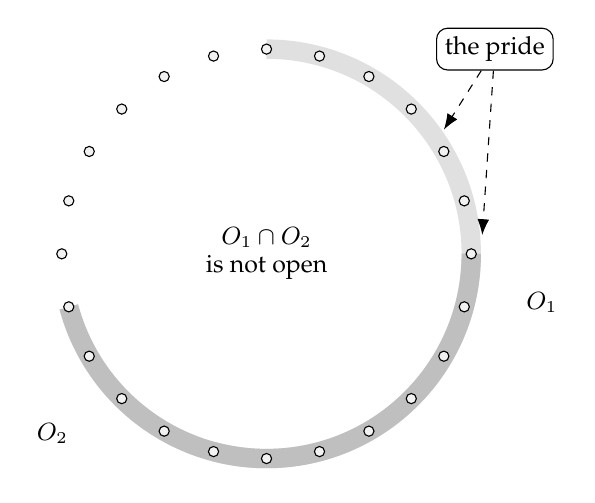
\begin{tikzpicture}[scale=1.0]
\foreach \i in {0,...,23} {
  \pgfmathsetmacro{\ang}{90 - \i*15}
  \node[circle,draw,inner sep=1.3pt,fill=black!5] (a\i) at (\ang:2.6) {};
}
\begin{scope}[on background layer]
  \draw[line width=7pt,black!12] (90:2.6) arc (90:-105:2.6);
  \draw[line width=7pt,black!25] (0:2.6) arc (0:-165:2.6);
\end{scope}
\node at (-10:3.55) {\small $O_1$};
\node at (-140:3.55) {\small $O_2$};
\node[align=center] at (0,0) {\small $O_1 \cap O_2$\\[-2pt]\small is not open};
\node[draw,rounded corners,inner sep=3pt] (pride) at (2.9,2.6)
  {\small the pride};
\draw[-{Latex[length=2mm]},dashed] (pride) -- (35:2.75);
\draw[-{Latex[length=2mm]},dashed] (pride) -- (5:2.75);
\end{tikzpicture}
\caption{The herd as a semitopology. Arcs of length at least $k$ are the basis
of $\Open$; their union is open, their intersection in general is not. The
pride observes participants one at a time, paying for each.}
\label{fig:ring}
\end{figure}

\subsection{The pride's ladder}

Seven hypotheses, priced on the schedule $\kappa(d) = 2^d$ per candidate
examined \cite{game}: a heading costs $2$ (spatial, depth one), a deposited
confidence costs $4$ (spatial, depth two), testing one open costs a further $4$
(the modal step), and driving the population forward one tick costs $8$.
Observations are cached within a single evaluation, so no participant is billed
twice for one verdict.

\begin{enumerate}[label=R\arabic*.,leftmargin=2.2em]
\setcounter{enumi}{-1}
\item $\top$. No theory; commit at random.
\item One heading. Read a single animal.
\item Sample of five. Read five animals; take the sign of the sum.
\item Crisp $\Ebox$. Is there an actionable coalition uniformly heading one
      way? Since a union of basis arcs is uniform iff each constituent is, it
      suffices to test the $N$ arcs of length exactly $k$.
\item Graded $\gE{\Nsp}{\Val}$ over the quorum algebra of
      Definition~\ref{def:quorum}, returning value and witness.
\item Topen member. Read one animal of a known topen and its confidence;
      predict the whole topen.
\item $\nu$: drive the population forward six sweeps and then apply R4. This is
      the fixed point of Remark~\ref{rem:twomod} evaluated by simulation
      instead of by inspection.
\end{enumerate}

R0--R2 and R5 are \emph{perception}: they read structure the herd has already
computed. R3--R4 are perception at modal depth one. R6 is \emph{driving}. The
read-versus-drive distinction of \cite{game} is thus laid out along the ladder,
and the pricing schedule is what makes the comparison mean anything.

\subsection{The ladder measured}\label{sec:ladder}

\begin{table}[t]
\centering
\begin{tabular}{@{}lrrrrr@{}}
\toprule
rung & coverage & precision & accuracy & cost & return\\
\midrule
R0 $\top$                  & $1.0000$ & $0.4985$ & $0.4985$ & $0.0$    & ---\\
R1 one heading             & $1.0000$ & $0.9002$ & $0.9002$ & $2.0$    & $+0.20087$\\
R5 topen member            & $0.8498$ & $0.9744$ & $0.9031$ & $4.0$    & $+0.00144$\\
R2 sample of five          & $1.0000$ & $0.9868$ & $0.9868$ & $10.0$   & $+0.01394$\\
R3 crisp $\Ebox$           & $0.7510$ & $1.0000$ & $0.8755$ & $190.2$  & $-0.00062$\\
R4 graded $\gE{\Nsp}{\Val}$& $0.7510$ & $1.0000$ & $0.8755$ & $192.0$  & $+0.00000$\\
R6 $\nu$ drive forward     & $1.0000$ & $0.9832$ & $0.9832$ & $1344.0$ & $+0.00009$\\
\bottomrule
\end{tabular}
\caption{The ladder, ordered by cost. $k = 13$, observation at $t = 90$, $4000$
stampedes that reached a conclusion. \emph{Coverage} is the fraction of trials
on which the rung issues a verdict at all; \emph{precision} is its accuracy
given that it does; \emph{accuracy} folds the two together by tossing a coin on
$\bv$, which is what an animal that must commit actually does. \emph{Return} is
the marginal gain in accuracy per metered unit against the next cheaper rung.}
\label{tab:ladder}
\end{table}

Read naively, Table~\ref{tab:ladder} says the coalition rungs are a bad
purchase: R3 has \emph{negative} marginal return, costs nineteen times what R2
costs, and has lower folded accuracy. This replicates the headline of
\cite{game} --- yield, not truth --- and if that were the end of it the note
would be reporting that Coalition Logic is ecologically worthless.

It is not the end of it. The folded accuracy column is the wrong instrument.

\subsection{Lean versus commitment}\label{sec:leanvscommit}

R2 and R3 answer different questions. A five-animal sample reports which way the
herd is \emph{leaning}. The coalition modality reports that it has
\emph{committed}. A lean can reverse; a decided coalition, under twinedness,
cannot.

\begin{table}[t]
\centering
\begin{tabular}{@{}rrrrr@{}}
\toprule
$t$ & sample coverage & sample precision & coalition coverage & coalition precision\\
\midrule
$30$  & $1.0000$ & $0.9160$ & $0.0037$ & $1.0000$\\
$50$  & $1.0000$ & $0.9640$ & $0.1263$ & $1.0000$\\
$70$  & $1.0000$ & $0.9797$ & $0.4740$ & $1.0000$\\
$90$  & $1.0000$ & $0.9837$ & $0.7527$ & $1.0000$\\
$120$ & $1.0000$ & $0.9873$ & $0.9223$ & $1.0000$\\
\bottomrule
\end{tabular}
\caption{The coalition modality trades coverage for precision. $3000$
stampedes; $k = 13$. Across all five observation times the coalition rung
issued $6839$ verdicts and got every one of them right.}
\label{tab:lean}
\end{table}

\begin{observation}[What the modality buys]\label{obs:irrev}
Over $6839$ coalition verdicts, precision was $1.0000$ at every observation
time, including at $t = 30$ where coverage is $0.37\%$. The sample majority,
which always answers, was wrong on $8.4\%$ of its verdicts at $t=30$ and on
$1.3\%$ at $t = 120$.
\end{observation}

So the coalition rung is not a worse predictor of direction; it is a different
instrument. It converts a probabilistic lean into a categorical commitment,
paying for the conversion in coverage and in tokens. For a pride the
distinction is the whole game: a charge committed on a lean that then reverses
is worse than no charge at all, because the pride has spent its ambush.

\begin{remark}[The verdict is not a theorem]
Precision $1.0000$ is measured, not proved. With $\varepsilon > 0$ the dynamics
can in principle unwind a decided coalition, and nothing in
Proposition~\ref{prop:functional} forbids it: twinedness rules out two
\emph{simultaneous} conclusions, not a later reversal of one. What the
measurement shows is that under this dynamics the event did not occur in $6839$
opportunities. A general statement would need a hypothesis relating the noise
rate to the coalition size, and is left open (Q\ref{q:irrev}).
\end{remark}

\begin{principle}[A second currency]\label{prin:currency}
The yield metric of \cite{game} --- accuracy gained per metered unit --- prices
instruments that always answer. It systematically underprices instruments whose
value is that they sometimes decline to. Coverage and precision must be
reported separately, and an ecology in which commitment is irreversible will
pay for precision at prices the yield metric calls irrational.
\end{principle}

\subsection{Earliness}

\begin{table}[t]
\centering
\begin{tabular}{@{}lrrrrrrr@{}}
\toprule
rung & $t{=}20$ & $40$ & $60$ & $80$ & $100$ & $140$ & first $\ge 0.80$\\
\midrule
R0 $\top$          & $0.486$ & $0.492$ & $0.512$ & $0.519$ & $0.509$ & $0.492$ & ---\\
R1 one heading     & $0.623$ & $0.705$ & $0.818$ & $0.868$ & $0.915$ & $0.949$ & $60$\\
R2 sample of five  & $0.845$ & $0.948$ & $0.975$ & $0.986$ & $0.983$ & $0.981$ & $20$\\
R3 crisp $\Ebox$   & $0.500$ & $0.518$ & $0.657$ & $0.813$ & $0.920$ & $0.974$ & $80$\\
R4 graded          & $0.500$ & $0.518$ & $0.657$ & $0.813$ & $0.920$ & $0.974$ & $80$\\
R5 topen member    & $0.587$ & $0.693$ & $0.791$ & $0.861$ & $0.914$ & $0.951$ & $70$\\
R6 $\nu$           & $0.938$ & $0.966$ & $0.983$ & $0.981$ & $0.985$ & $0.987$ & $10$\\
\bottomrule
\end{tabular}
\caption{Folded accuracy against observation time, and the earliest sampled time
at which each rung reaches $0.80$. $1200$ stampedes.}
\label{tab:early}
\end{table}

R6, which drives the population forward, is the earliest instrument by a wide
margin: it is at $0.938$ when every perceptual rung is near chance. This is what
a lookahead buys, and it is also why it costs $1344$ units against R2's $10$.
The ecological reading of Table~\ref{tab:early} is that simulation is a
luxury good: it is genuinely the best instrument on the board, and almost
nothing can afford it. The identity of the R3 and R4 rows is
Remark~\ref{rem:brittle} made visible.

\section{The counter-move}\label{sec:countermove}

Nothing so far has given the herd a say. But a population that is being read
has an interest in not being readable, and Principle~\ref{prin:safetyislegibility}
tells it exactly where to attack: break quorum intersection.

In the model this is done by inserting seams --- bonds of zero coupling ---
into the ring. A herd with enough seams cannot form an arc of length $k$ that
is internally uniform, because every such arc crosses a seam and the two sides
of a seam decide independently.

\begin{table}[t]
\centering
\begin{tabular}{@{}rrrr@{}}
\toprule
seams & $\Pr(\text{herd concludes})$ & pride coverage & pride precision\\
\midrule
$0$ & $0.7257$ & $0.7520$ & $0.9993$\\
$1$ & $0.6780$ & $0.6030$ & $1.0000$\\
$2$ & $0.4984$ & $0.3645$ & $0.9986$\\
$3$ & $0.2957$ & $0.3015$ & $1.0000$\\
$4$ & $0.4495$ & $0.0910$ & $1.0000$\\
$5$ & $0.2877$ & $0.0685$ & $1.0000$\\
$6$ & $0.2331$ & $0.0115$ & $1.0000$\\
\bottomrule
\end{tabular}
\caption{Cohesion against legibility. $k = 13$, observation at $t = 90$. As the
herd fragments its own quorum structure, the pride's coverage collapses by a
factor of $65$ while its precision does not move.}
\label{tab:seams}
\end{table}

\begin{observation}[Illegibility is denial of liveness, not induction of error]
\label{obs:liveness}
Across Table~\ref{tab:seams} the pride's precision stays within
$[0.9986, 1.0000]$ while its coverage falls from $0.7520$ to $0.0115$. The herd
does not make the pride wrong. It makes the pride silent.
\end{observation}

This is exactly the signature of a consensus failure seen from the far side.
An adversary who breaks quorum intersection in Paxos does not cause two correct
replicas to decide differently --- that is what the intersection property is
there to prevent, and the property is not what the adversary can touch. The
adversary causes the protocol to \emph{stop deciding}. Safety is preserved,
liveness is lost. Read from outside, the same event is an observer that keeps
being right and stops being able to say anything.

\begin{corollary}[The price of illegibility]\label{cor:pricecounter}
The herd pays for the pride's silence in its own coordination: across the same
rows, the probability that the herd reaches any conclusion at all falls from
$0.7257$ to $0.2331$. A herd that cannot be read is a herd that cannot decide
which way to run.
\end{corollary}

\begin{principle}[The legibility trade]\label{prin:trade}
For a population under observation, the safety--liveness trade-off of consensus
and the cohesion--illegibility trade-off of predation are one trade-off. A
population buys privacy with the same currency it buys agreement, and cannot
spend it twice.
\end{principle}

Principle~\ref{prin:trade} is the note's second payoff from the reversal, and
the one that seems most likely to generalise beyond herds. It is a claim about
any population whose members must coordinate while being observed by something
that profits from predicting them, which is a wide class.

\begin{remark}[Dual use]
Read as engineering rather than ecology, Principle~\ref{prin:trade} says that a
protocol cannot be made unobservable by weakening its quorum structure without
losing exactly the liveness that quorum structure was providing. Privacy
mechanisms that work by fragmenting agreement are paying for it in the
protocol's own progress, and the exchange rate is the one in
Table~\ref{tab:seams}.
\end{remark}

\section{Compression: what a topen is worth}\label{sec:topen}

A topen is a transitive open: an open $T$ such that any two opens meeting $T$
meet each other. Gabbay's theory makes topens the pivotal notion because their
members are guaranteed to decide alike. For an observer this is a compression
result.

\begin{principle}[One observation buys $n$ predictions]\label{prin:compress}
If $T$ is a topen and $q \in T$, then observing $q$ determines the observer's
prediction for every member of $T$. The value of the observation is multiplied
by $|T|$, and the observer's optimal strategy is to spend on \emph{identifying
topens} rather than on observing members.
\end{principle}

Measured in a two-cluster herd (seams at positions $0$ and $N/2$, so the two
half-rings decide independently and each is a topen):

\begin{center}
\begin{tabular}{@{}lrr@{}}
\toprule
 & agreement with the observed animal & predictions per observation\\
\midrule
same cluster & $0.8683$ & $6.5$\\
across the seam & $0.5606$ & $5.9$\\
\bottomrule
\end{tabular}
\end{center}

Inside the topen a single observation yields $6.5$ predictions at $86.8\%$
accuracy --- $4.81$ correct net of errors. Across the seam the same observation
yields nothing above chance. The entire value of the observation is
concentrated in the topen, and an observer that has misidentified the topen
boundary is paying for information it is not receiving.

\begin{remark}[Why topen identification is the expensive part]
Identifying a topen is a question about \emph{pairs} of opens, so its evaluation
is quadratic in the basis where checking a single coalition is linear. This is
the observer's version of the fact that transitivity is the expensive axiom.
It is also where the ultrametric confinement of
\cite[Prop.~Confinement]{scientist} bites hardest: a topen boundary in the wrong
place is a shape error, and shape errors are not reachable by refinement.
\end{remark}

\section{The margin is a clock}\label{sec:clock}

Remark~\ref{rem:brittle} left the grading looking useless: at $k = 13$ it
returns exactly what the crisp modality returns. The resolution is that the
observer should not evaluate the graded formula at the coalition size it cares
about. It should evaluate a \emph{relaxed} formula --- coalitions of size
$k_{\mathrm{warn}} = 7$ --- purely as an early-warning instrument, while
retaining $k = 13$ as the definition of commitment.

Conditioning on stampedes that have \emph{not} committed at $t = 60$, and
banding by the tropical margin of the relaxed formula:

\begin{table}[t]
\centering
\begin{tabular}{@{}lrrr@{}}
\toprule
margin quartile & mean margin & ticks to commitment & direction correct\\
\midrule
lowest  & $0.0864$ & $42.4$ & $0.6080$\\
second  & $0.7648$ & $29.6$ & $1.0000$\\
third   & $0.8000$ & $28.9$ & $1.0000$\\
highest & $0.9872$ & $18.0$ & $1.0000$\\
\bottomrule
\end{tabular}
\caption{The relaxed margin as an early-warning signal. $1500$ stampedes
uncommitted at $t = 60$, $k = 13$, $k_{\mathrm{warn}} = 7$.}
\label{tab:clock}
\end{table}

\begin{observation}[What grading buys]\label{obs:clock}
The margin is monotone in both columns that matter: time to commitment falls
from $42.4$ to $18.0$ ticks across the quartiles, and directional correctness
rises from $0.6080$ to $1.0000$. A crisp verdict at $k=13$ says only ``not
yet''. The relaxed graded value says how long ``not yet'' will last.
\end{observation}

For a pride this is the difference between knowing that the herd is undecided
and knowing that it has eighteen ticks to get into position. Grading does not
improve the answer to \emph{which way}; it answers \emph{when}, which is a
question the crisp logic cannot ask.

The swarm shows the same shape, and there the quantity is one field workers
already record. Conditioning on episodes undecided at $t = 250$ with a mild
quality disparity, and banding by the advocacy margin between the two sites:

\begin{center}
\begin{tabular}{@{}lrr@{}}
\toprule
margin quartile & mean margin & ticks to quorum\\
\midrule
lowest  & $0.1016$ & $59.7$\\
second  & $0.3009$ & $35.1$\\
third   & $0.4625$ & $18.4$\\
highest & $0.5914$ & $8.4$\\
\bottomrule
\end{tabular}
\end{center}

A sevenfold spread in the wait, read off a quantity that costs nothing extra to
observe. For a swarm this is the difference between a cluster that should be
warming up and one that should not; for a pride it is the difference between
getting into position and wasting an ambush.

\begin{principle}[Two dials]\label{prin:twodials}
The value algebra and the coalition size must be varied together. Grading at
the operative coalition size is crisp in disguise
(Remark~\ref{rem:brittle}); relaxing without grading gives an unreliable crisp
verdict (the lowest quartile of Table~\ref{tab:clock} is right only $60.8\%$ of
the time); relaxing \emph{and} grading gives a graded verdict about a weaker
proposition, which is the useful object.
\end{principle}

Principle~\ref{prin:twodials} connects the two lattices that have been running
in parallel throughout: the relaxation lattice of \cite{scientist}, which orders
hypotheses by logical strength, and the algebra table of
\cite{gradedwhere,choicef}, which orders resolutions by what they can express.
They are not independent knobs, and a note that turned only one of them would
have concluded that grading buys nothing.

\section{Altitude: where this sits in the choice hierarchy}\label{sec:altitude}

The formulae of this note are clauses, and \cite{choicef} assigns clauses a
choice type $\chi$ --- a bound on the Weihrauch degree of the resolver a clause
demands. It is worth locating the coalition modality on that lattice, because
doing so predicts what a real observer can afford.

\begin{proposition}[The coalition modality is a width engine]\label{prop:width}
Over a presented basis, $\gE{\Nsp}{\Val}$ is a finite $\bigoplus$ and carries
choice type $\bot$: its value is computed by inspection with no oracle. When
the basis is a family indexed by a countable presented set, the modality is the
\emph{width} engine of \cite[\S5]{choicef}, of degree $\mathrm{C}_{\mathbb{N}}$
when the index is $\mathbb{N}$ and $\mathrm{C}_{2^{\mathbb{N}}} \equiv
\mathrm{WKL}$ when the index is a powerset.
\end{proposition}

\begin{proposition}[Coherence is a depth engine]\label{prop:depth}
$\Phi_{\mathrm{coh}} = \nu X.\gE{\Nsp}{\Val}(\lceil\beta\rceil \otimes
\gK{}{}X)$ is a greatest fixed point over the run tree and is therefore the
\emph{depth} engine, of degree $\mathrm{WKL}$; its content is compactness.
\end{proposition}

\begin{corollary}[Exact herd-reading is expensive]\label{cor:expensive}
Predicting that a population will \emph{continue} to agree combines both
engines, which are Weihrauch-incomparable \cite[\S5]{choicef}, and so sits at
$\mathrm{C}_{\mathbb{N}^{\mathbb{N}}}$ or above.
\end{corollary}

\begin{remark}[And so real prides do not do it]
Corollary~\ref{cor:expensive} is not merely a complexity remark; combined with
the pricing schedule it is a prediction about behaviour, and
Table~\ref{tab:ladder} bears it out. R6, the only rung that evaluates anything
resembling $\Phi_{\mathrm{coh}}$, costs $1344$ units against R2's $10$. The
instruments that survive an ecological budget are the ones that read structure
the herd has already deposited --- headings, confidences, arcs --- which is the
read-versus-drive thesis of \cite{game} arriving from the direction of degree
theory rather than of measurement. A pride does not simulate zebra. It looks at
their necks.
\end{remark}

\begin{remark}[Strong fairness, again]
The identification of $\nu$-over-the-run-tree with $\mathrm{WKL}$ is the same
identification that gave strong fairness its degree in \cite{choicef}, where the
content of the weak/strong fairness gap turned out to be compactness. The
present note adds a third instance of the same pattern: the gap between ``some
coalition agrees now'' and ``some coalition keeps agreeing'' is the same gap.
\end{remark}

\subsection{Subject reduction, and the same suspect}

\begin{question}[Subject reduction for coalition clauses]\label{q:sr}
Does a shard whose clauses mention $\gE{\Nsp}{\Val}$ have invariant choice
types under reduction?
\end{question}

The answer is expected to be no, for the reason it was no in \cite{choicef}.
Reduction substitutes a quoted process for a name and $*y$ drops an arbitrary
received process into term position, so a clause whose declared coalition
structure is finitely presented can, after one communication, come to mention a
received process carrying a $\nu$ over a non-presented $\Open$. Strength is
mailed in. The repair is the same: a stratified \emph{where}, declaring a
ceiling and checking levels on drops. Reflection is now the suspect in a fourth
place, and Krivine's observation that $\mathrm{DC}$ is realised by adding a
\texttt{quote} instruction to the machine remains the sharpest statement of why:
the rho calculus has had its choice primitive in the syntax since \cite{Mer05}.

\section{What is shown and what is not}\label{sec:shown}

\paragraph{Shown.} That Coalition Logic admits an observational reading which
needs only its model theory (Proposition~\ref{prop:pf-free}); that the
participant/process-structure distinction of \cite[\S7.1]{consensus} collapses
under reflection (Proposition~\ref{prop:collapse}); that the correct value
algebra for a quorum is $\min$-based and that this is the fragment where the
observer receives a witness (Propositions~\ref{prop:decay},
\ref{prop:witness}); that a mortal observer conflates fault with poverty
(Proposition~\ref{prop:twobottoms}, Table~\ref{tab:bottom}); that quorum
intersection is what makes a hypothesis about a population well posed
(Proposition~\ref{prop:functional}); and, by measurement in one model, that the
coalition modality trades coverage for precision (Table~\ref{tab:lean}), that a
population's counter-move costs the observer liveness rather than accuracy
(Table~\ref{tab:seams}), that topen membership is where the value of an
observation is concentrated (\S\ref{sec:topen}), and that the relaxed graded
margin is an early-warning clock (Table~\ref{tab:clock}).

From the swarm: that quorum sensing rather than consensus sensing is forced by
the access grades (Proposition~\ref{prop:whyquorum}, Corollary~\ref{cor:forced});
that two simultaneous quorums require $2k$ scouts and hence that takeoff with
dissent is confined to swarms with $S \ge 2k$ (Theorem~\ref{thm:twok}); that
cross inhibition's duty changes at that same threshold
(Principle~\ref{prin:jobs}, Observation~\ref{obs:jobswitch}); and that under
encounter sensing quorum errors are one-sided with the apparent threshold
scaling in cavity geometry (Proposition~\ref{prop:onesided},
Corollary~\ref{cor:notanumber}).

\paragraph{Not shown.} That any swarm prediction has been \emph{tested};
E1--E6 of \S\ref{sec:protocol} are proposals, and the simulated tables show
only that the predictions are non-vacuous in a model with the right mechanisms
in it. That the advocacy-set reading of $\Open$ is the right one rather than
the site-occupancy reading --- E6 is precisely the experiment that would tell
them apart, and Theorem~\ref{thm:twok} holds under either. That the framework
improves on the accumulator models in any respect they address; it does not,
and \S\ref{sec:swarm} says so at the outset. That precision $1.0000$ for the
coalition modality is
anything but an artefact of this dynamics at this noise rate
(Q\ref{q:irrev}). That the pricing schedule $\kappa(d) = 2^d$ is the right one
--- it is inherited from \cite{game}, where it was already flagged as a choice,
and the qualitative shape of Table~\ref{tab:ladder} is robust to varying it
while the boundaries are not. That a ring with arcs is a good model of a herd;
it is a good model of a semitopology that is not a topology, which is what was
needed. That the observer's guessed $\Open$ can be learned efficiently --- the
note assumes a guess and prices its use, and says nothing about acquiring it
beyond the negative result inherited from ultrametric confinement. That any of
this extends to $n$-twinedness for $n > 2$, which is where heterogeneous quorum
systems live and where the interesting engineering is.

\paragraph{Deliberately not attempted.} The resolutive reading --- using a
population's consensus to settle a race inside the observer --- is not developed
here. Remark~\ref{rem:weighnotselect} says why it is the harder direction: it
requires a section where the clause provides only a weighting. It remains an
interesting direction and is the natural next note.

\section{Open problems}\label{sec:open}

\begin{question}[Irreversibility]\label{q:irrev}
Give a condition on the noise rate, the coalition size and the neighbourhood
structure under which a decided coalition is stable with probability one, so
that Observation~\ref{obs:irrev} becomes a theorem rather than a measurement.
\end{question}

\begin{question}[Learning $\Open$]
Principle~\ref{prin:inversion} says the semitopology is the hypothesis. Give a
revision procedure over guessed semitopologies, priced, and locate it on the
ultrametric: which errors in $\Open$ are refinement-reachable and which are
shape errors requiring recombination?
\end{question}

\begin{question}[Heterogeneous quorums]
Extend the worked example from $2$-twinedness on a ring to genuinely
heterogeneous quorum systems, where different participants have different
notions of an actionable coalition. This is where Gabbay's theory has its real
content and where Corollary~\ref{cor:legibility} becomes a statement about
\emph{whose} question is well posed.
\end{question}

\begin{question}[The compatibility relation as an observation]
Semiframes replace intersection by a compatibility relation $*$, read in
\cite{realizability} as co-realizability: $\varphi$ and $\psi$ share a witness.
What does an observer pay to test $A * B$, and is the compatibility relation
cheaper to observe than the coalitions themselves? If so, an observer should
work in the semiframe rather than the semitopology.
\end{question}

\begin{question}[The cost of cross inhibition]
Table in \S\ref{sec:twok} suggests cross inhibition buys decisiveness partly by
suppressing correct advocacy, choosing the better site slightly less often at
moderate disparity. Is this an artefact of the implementation, and if not, what
is the swarm's optimal $\sigma$ as a function of $S/k$ and site disparity?
\end{question}

\begin{question}[Which $\Open$ do the bees act on?]
Observation~\ref{obs:switchers} takes the basis of $\Open$ to be advocacy sets,
which makes switchers the reason the meet fails. Site occupancies would give a
different and nearly-degenerate structure. E6 of \S\ref{sec:protocol}
distinguishes them empirically; is there an argument from cost that picks one
in advance, as Corollary~\ref{cor:forced} picks the quorum formula?
\end{question}

\begin{question}[Composition of observers]
Two prides watching one herd are two learners with overlapping namespaces in
the sense of \cite{compose}. The competitive dilution result there says each
retains a share of the deep inquiry it could afford alone. Does watching a
population deplete it as a source, and if so is the herd a rate-limited source
or a prey item in the trophic sense of \cite[\S10]{scientist}?
\end{question}

\begin{question}[Stochastic evaluation]
Section 7.2 of \cite{consensus} proposes expressing Coalition Logic axioms as
MeTTaIL rewrite rules and using the weighted-GSLT machinery of \cite{weighted}
to explore probabilistic consensus. The graded modality of
Definition~\ref{def:gE} is a natural key for a weight map. Does the partition
discipline of \cite[\S3]{weighted} survive keys mentioning $\gE{\Nsp}{\Val}$,
given that requirement R3 there restricts keys to structural formulae?
\end{question}

\begin{question}[The second currency]
Principle~\ref{prin:currency} asserts that coverage and precision must be
priced separately. Give the ecology in which precision is worth its cost: a
game in which a reversed commitment is strictly worse than no commitment, and
compute the exchange rate at which R3 invades a population of R2 players.
\end{question}

\section{Conclusion}

The companion note asked how to build a coalition from a proof. This one asks
how to notice that one has formed. The machinery is the same --- Gabbay's
modality, the rho calculus, the join --- but running it in the observational
direction changes what is hard and what is easy. The proof theory that blocks
synthesis is not needed; the model theory that exists suffices. What becomes
hard instead is everything the synthesis reading takes for granted: which
sub-populations can act as one, whether the observer can afford to find out, and
whether a verdict of ``don't know'' is a fact about the world or about the
purse.

The two examples are not two illustrations of one point. The swarm is the case
where the observer is a participant and its verdict is the decision, so the
clause and the resolver appear together and the theory has to say how they are
kept apart; the swarm keeps them apart by putting them in different bees. The
pride is the case where the observer has no purchase at all, so the theory has
to say what watching alone can buy; the answer is irreversibility, bought with
coverage, at a price the ordinary yield metric calls irrational. Neither case
would have produced the other's result.

Three things came out of the work that were not put in. The first is that
quorum intersection, which consensus theory keeps for safety, is what makes a
population legible from outside at all --- and in the swarm it acquires a number,
$S \ge 2k$, that says which swarms are able to disagree with themselves. The
second is that a population resists being read by denying coverage rather than
by inducing error, and pays for the resistance in its own capacity to agree, so
that privacy and coordination are drawn from one account. The third is smaller
and more uncomfortable: an observer poor enough sees a world full of broken
things, because a participant it could not afford to examine and a participant
that is genuinely stuck return the same value. In the swarm that has a shape ---
scouts should fail to see quorums that are there, and never see quorums that
are not --- and it means the number a field biologist writes down as the quorum
threshold is partly a fact about the bee and partly a fact about the box. That
last point is not about bees. It is about anything that has to pay to look.

\appendix

\section{The pride and the herd in rholang}\label{app:rholang}

The listing below is the population and the observer as rho processes, in the
variant of rholang carrying \emph{where}-clauses. Names are manufactured by
quotation rather than bound by \texttt{new} where the freshness argument of
\cite[\S3]{scientist} applies; \texttt{new} is retained where it reads better
and is sugar. Guards written in the ideal logic rather than the implemented
fragment are marked \texttt{//! ideal}.

\begin{lstlisting}
new herd, pride, tick in {

  // ---- a participant -------------------------------------------------
  // animal k lives at the manufactured name @[*herd, k]; it holds its
  // heading as a resting send and re-deposits it after each update.

  contract @[*herd, "animal"](@k) = {
    for (@h <- @[*herd, k]) {
      // read the window; couplings are data on the bond channels
      for (@w <- @[*herd, "window", k]) {
        match w {
          tot => {
            // the deposit: heading AND the confidence the neighbourhood
            // has already computed. This is what makes perception cheap.
            @[*herd, k]!(if (tot > 0) 1 else if (tot < 0) -1 else h) |
            @[*herd, "conf", k]!(agree(w) / total(w))
          }
        }
      }
    }
  } |

  // ---- an open set ----------------------------------------------------
  // an arc of length K starting at a is presented as a name predicate;
  // testing it is a join over its members, which is the coalition
  // modality's term-level shadow read in the observation direction.

  contract @[*pride, "arcUniform"](@a, @K, @d, ret) = {
    new acc in {
      acc!(true, 0) |
      for (@ok, @i <= acc) {
        if (i == K) { ret!(ok) }
        else {
          for (@h <<- @[*herd, (a + i) % 24]) {   // peek, not consume
            acc!(ok and (h == d), i + 1)
          }
        }
      }
    }
  } |

  // ---- the crisp coalition modality ------------------------------------
  // exists O in Open. p in O and all q in O have heading d.
  // A union of basis arcs is uniform iff each arc is, so the N arcs of
  // length exactly K exhaust the test.

  contract @[*pride, "Ebox"](@d, ret) = {
    new scan, hit in {
      scan!(0) |
      for (@a <= scan) {
        if (a == 24) { ret!(false) }
        else {
          new r in {
            @[*pride, "arcUniform"]!(a, 13, d, *r) |
            for (@u <- r) { if (u) { ret!(true) } else { scan!(a + 1) } }
          }
        }
      }
    }
  } |

  // ---- the graded coalition modality -----------------------------------
  // <E>_V psi = max over opens O of min over q in O of psi(q).
  // The witness arc is returned alongside the value: Prop 12 says the
  // value is attained, and the pride charges at the witness, not the value.

  contract @[*pride, "gradedE"](@d, ret) = {
    new scan in {
      scan!(0, 0.0, -1) |
      for (@a, @best, @arg <= scan) {
        if (a == 24) { ret!(best, arg) }
        else {
          new m in {
            @[*pride, "arcMin"]!(a, 13, d, *m) |
            for (@v <- m) {
              if (v > best) { scan!(a + 1, v, a) } else { scan!(a + 1, best, arg) }
            }
          }
        }
      }
    }
  } |

  // ---- the observer ----------------------------------------------------
  // the hypothesis sits in the where-clause. The pride commits when the
  // graded value clears zero, and charges at the witness arc.

  for (@t <- tick) {
    new v in {
      @[*pride, "gradedE"]!(1, *v) |
      for (@val, @arc <- v where val > 0.0) {     //! ideal: <E>_N psi
        @[*pride, "commit"]!("right", arc)
      }
    }
  }
}
\end{lstlisting}

Two conventions are worth flagging. The peek \texttt{<<-} rather than the
linear receive \texttt{<-} is what makes the scan \emph{perception} rather than
\emph{interaction}: a linear receive would consume the animal's heading, which
is to say the pride would move the zebra by looking at it. The separation is
the same one forced in \cite[\S4.3]{game}, where threat markers had to live on
their own names lest perception rendezvous with the move channel and play the
move. Grade one and grade two of access are kept apart by choice of namespace,
and that is the only mechanism available.

\section{The computations}\label{app:computations}

All numbers are produced by \texttt{swarm.py} and \texttt{herd.py} (standard
library only, single seed $20260813$ in each). Run \texttt{python3 swarm.py}
and \texttt{python3 herd.py}.

\paragraph{Parameters.} $N = 24$ participants; window radius $W = 2$; per-update
noise $\varepsilon = 0.03$; horizon $400$ ticks; seam coupling $0$, elsewhere
$1$. A stampede counts as concluding when the final total heading exceeds
$N/2$ in magnitude.

\paragraph{Pricing.} $\kappa(d) = 2^d$ per candidate examined: a heading costs
$2$, a deposited confidence costs $4$, a tested open costs a further $4$, and
one tick of driving costs $8$. Observations are cached within a verdict.

\subsection*{The swarm: \texttt{swarm.py}}

\paragraph{Parameters.} $S$ scouts, two cavities, quorum threshold $k = 15$;
per-tick independent discovery $\nu = 0.0060$, recruitment coefficient
$\rho = 0.0500$ applied to $q_i D_i / S$, quality-independent abandonment
$\alpha = 0.0050$, cross-inhibition strength $\sigma = 0.0200$ when enabled;
piping window $60$ ticks, horizon $1500$ ticks, $1000$ episodes per cell, seed
$20260813$. A site reaching quorum locks its scouts, since piping bees neither
abandon nor can be stopped; this is what makes the counting argument of
Theorem~\ref{thm:twok} bind on the simulation as well as on the biology.

\paragraph{The measurements.}
\begin{enumerate}[leftmargin=1.6em]
\item \texttt{structural\_threshold} --- split, deadlock and clean-decision
      rates against $S$, with and without cross inhibition, equal cavities
      (Table~\ref{tab:twok}).
\item \texttt{unequal\_sites} --- the same against site disparity at $S = 40$
      (\S\ref{sec:twok}).
\item \texttt{one\_sided\_errors} --- false negative and false positive rates
      under encounter sensing, and the apparent threshold in true bees, against
      effective cavity area (\S\ref{sec:onesided}).
\item \texttt{margin\_clock} --- the advocacy margin as a predictor of the wait
      to quorum (\S\ref{sec:clock}).
\end{enumerate}

\paragraph{What the simulation is and is not.} It is a standard
discovery--recruitment--abandonment--inhibition scheme, chosen so that the
mechanisms named in the text are present and none other is. It is not
calibrated against field data and its rate constants are not estimates of
anything. Its only jobs are to confirm that the structural floor of
Theorem~\ref{thm:twok} is respected, to show that the predictions of
\S\ref{sec:twok} and \S\ref{sec:onesided} are non-vacuous, and to give the
regime table numbers.

\subsection*{The herd: \texttt{herd.py}}

\paragraph{The measurements.}
\begin{enumerate}[leftmargin=1.6em]
\item \texttt{ladder} --- coverage, precision, folded accuracy and mean cost per
      rung; $4000$ concluding stampedes (Table~\ref{tab:ladder}).
\item \texttt{reversal} --- coverage and precision of the sample and coalition
      verdicts at five observation times; $3000$ stampedes
      (Table~\ref{tab:lean}).
\item \texttt{twinedness\_witness} --- the constructed split state deciding both
      directions at $k = 12$, and the exhaustive check over all $24\times24$ arc
      pairs that no two arcs of length $13$ are disjoint
      (Observation~\ref{obs:twozeros}).
\item \texttt{earliness} --- folded accuracy against observation time;
      $1200$ stampedes (Table~\ref{tab:early}).
\item \texttt{twinedness} --- the ambiguity transition in $k$; $2500$ stampedes
      per row (Table~\ref{tab:twined}).
\item \texttt{cohesion\_vs\_legibility} --- conclusion probability, observer
      coverage and observer precision against seam count
      (Table~\ref{tab:seams}).
\item \texttt{budget\_confusion} --- the two bottoms; $2500$ stampedes
      (Table~\ref{tab:bottom}).
\item \texttt{topen\_multiplier} --- agreement inside and across a seam,
      unconditioned on the herd concluding; $3000$ stampedes
      (\S\ref{sec:topen}).
\item \texttt{margin\_predicts\_commitment} --- the relaxed margin as a clock;
      $1500$ stampedes uncommitted at $t = 60$ (Table~\ref{tab:clock}).
\end{enumerate}

\paragraph{A negative result worth keeping.} The first version of measurement 9
evaluated the graded modality at the operative coalition size $k = 13$ and
returned a margin of exactly zero on every trial, because $\min$ over thirteen
participants is zeroed by one dissenter. That failure is
Remark~\ref{rem:brittle}, and it is the reason Principle~\ref{prin:twodials}
is stated: the note would have concluded that grading buys nothing had the
coalition size not been relaxed alongside the algebra.

\begin{thebibliography}{99}

\bibitem[Cons]{consensus} L. G. Meredith. \emph{From Coalition Logic to Rho
Calculus: Toward a Curry--Howard Correspondence for Consensus Protocol
Synthesis}. Research Note, F1R3FLY, April 2026.

\bibitem[Sci]{scientist} L. G. Meredith. \emph{The Mortal Scientist: learning
as cost-accounted computation in a reflective higher-order calculus}. Research
Note, F1R3FLY, 2026.

\bibitem[Play]{game} L. G. Meredith. \emph{Learning to Play}. Research Note,
F1R3FLY, 2026.

\bibitem[Comp]{compose} L. G. Meredith. \emph{Composing Learners: populations as
namespaces, parallel composition as the operator}. Research Note, F1R3FLY, 2026.

\bibitem[GW]{gradedwhere} L. G. Meredith. \emph{Graded Where-Clauses}. Research
Note, F1R3FLY, 2026.

\bibitem[ChF]{choicef} L. G. Meredith. \emph{Choice Principles as Graded
Where-Clauses: one programming paradigm at every altitude of the Weihrauch
lattice}. Research Note, F1R3FLY, 2026.

\bibitem[WG]{weighted} L. G. Meredith. \emph{Weighted Graph-Structured Lambda
Theories: stochastic and quantum execution for MeTTaIL}. Research Note,
F1R3FLY, 2026.

\bibitem[CM]{costmonad} L. G. Meredith. \emph{Cost accounting as a monad}.
Manuscript, 2026.

\bibitem[Real]{realizability} L. G. Meredith. \emph{On the nature of logic:
composition through realizability and computational witnesses}. Manuscript,
2026.

\bibitem[See10]{Seeley10} T. D. Seeley. \emph{Honeybee Democracy}. Princeton
University Press, Princeton, 2010.

\bibitem[SB99]{SB99} T. D. Seeley and S. C. Buhrman. Group decision making in
swarms of honey bees. \emph{Behav.\ Ecol.\ Sociobiol.}, 45:19--31, 1999.

\bibitem[SV04]{SV04} T. D. Seeley and P. K. Visscher. Quorum sensing during
nest-site selection by honeybee swarms. \emph{Behav.\ Ecol.\ Sociobiol.},
56:594--601, 2004.

\bibitem[VS07]{VS07} P. K. Visscher and T. D. Seeley. Coordinating a group
departure: who produces the piping signals on honeybee swarms?
\emph{Behav.\ Ecol.\ Sociobiol.}, 61:1615--1621, 2007.

\bibitem[See12]{Seeley12} T. D. Seeley, P. K. Visscher, T. Schlegel, P. M.
Hogan, N. R. Franks and J. A. R. Marshall. Stop signals provide cross
inhibition in collective decision-making by honeybee swarms. \emph{Science},
335(6064):108--111, 2012.

\bibitem[Pai13]{Pais13} D. Pais, P. M. Hogan, T. Schlegel, N. R. Franks, N. E.
Leonard and J. A. R. Marshall. A mechanism for value-sensitive decision-making.
\emph{PLoS ONE}, 8(9):e73216, 2013.

\bibitem[Rei17]{Reina17} A. Reina, J. A. R. Marshall, V. Trianni and T. Bose.
Model of the best-of-$n$ nest-site selection process in honeybees.
\emph{Phys.\ Rev.\ E}, 95(5), 2017.

\bibitem[Gab23]{Gab23} M. J. Gabbay. Semitopology: a topological approach to
decentralised collaborative action. \emph{Journal of Logic and Computation},
35(5), 2025. arXiv:2303.09287.

\bibitem[Gab24]{Gab24} M. J. Gabbay. \emph{Semitopology: Decentralised
Collaborative Action via Topology, Algebra, and Logic}. College Publications,
London, 2024.

\bibitem[Gab25]{Gab25} M. J. Gabbay. Declarative distributed broadcast using
three-valued modal logic and semitopologies. arXiv:2512.21137, December 2025.

\bibitem[GZ25]{GZ25} M. J. Gabbay and L. Zanolini. A declarative approach to
specifying distributed algorithms using three-valued modal logic.
arXiv:2502.00892, February 2025.

\bibitem[CC01]{CC01} L. Caires and L. Cardelli. A spatial logic for concurrency
(Part I). \emph{Inf.\ Comput.}, 186(2):194--235, 2003.

\bibitem[CC04]{CC04} L. Caires and L. Cardelli. A spatial logic for concurrency
(Part II). \emph{Theor.\ Comput.\ Sci.}, 322(3):517--565, 2004.

\bibitem[Mer05]{Mer05} L. G. Meredith and M. Radestock. A reflective
higher-order calculus. \emph{Electr.\ Notes Theor.\ Comput.\ Sci.},
141(5):49--67, 2005.

\end{thebibliography}

\end{document}
